%% (Master) Thesis template
% Template version used: v1.4
%
% Largely adapted from Adrian Nievergelt's template for the ADPS
% (lecture notes) project.


%% We use the memoir class because it offers a many easy to use features.
\documentclass[11pt,a4paper,titlepage]{memoir}

%% Packages
%% ========

%% LaTeX Font encoding -- DO NOT CHANGE
\usepackage[OT1]{fontenc}

%% Babel provides support for languages.  'english' uses British
%% English hyphenation and text snippets like "Figure" and
%% "Theorem". Use the option 'ngerman' if your document is in German.
%% Use 'american' for American English.  Note that if you change this,
%% the next LaTeX run may show spurious errors.  Simply run it again.
%% If they persist, remove the .aux file and try again.
\usepackage[english]{babel}
\makeatletter\AtBeginDocument{\let\@elt\relax}\makeatother

%% Input encoding 'utf8'. In some cases you might need 'utf8x' for
%% extra symbols. Not all editors, especially on Windows, are UTF-8
%% capable, so you may want to use 'latin1' instead.
\usepackage[utf8]{inputenc}

%% This changes default fonts for both text and math mode to use Herman Zapfs
%% excellent Palatino font.  Do not change this.
\usepackage[sc]{mathpazo}

%% The AMS-LaTeX extensions for mathematical typesetting.  Do not
%% remove.
\usepackage{amsmath,amssymb,amsfonts,mathrsfs}

%% NTheorem is a reimplementation of the AMS Theorem package. This
%% will allow us to typeset theorems like examples, proofs and
%% similar.  Do not remove.
%% NOTE: Must be loaded AFTER amsmath, or the \qed placement will
%% break
\usepackage[amsmath,thmmarks]{ntheorem}

%% LaTeX' own graphics handling
\usepackage{graphicx}
\usepackage{rotating}


%% We unfortunately need this for the Rules chapter.  Remove it
%% afterwards; or at least NEVER use its underlining features.
\usepackage{soul}

%% This allows you to add .pdf files. It is used to add the
%% declaration of originality.
\usepackage{pdfpages}

%% Some more packages that you may want to use.  Have a look at the
%% file, and consult the package docs for each.
%% See the TeXed file for more explanations

%% [OPT] Multi-rowed cells in tabulars
%\usepackage{multirow}

%% [REC] Intelligent cross reference package. This allows for nice
%% combined references that include the reference and a hint to where
%% to look for it.
\usepackage{varioref}

%% [OPT] Easily changeable quotes with \enquote{Text}
%\usepackage[german=swiss]{csquotes}

%% [REC] Format dates and time depending on locale
\usepackage{datetime}

%% [OPT] Provides a \cancel{} command to stroke through mathematics.
%\usepackage{cancel}

%% [NEED] This allows for additional typesetting tools in mathmode.
%% See its excellent documentation.
\usepackage{mathtools}

%% [ADV] Conditional commands
%\usepackage{ifthen}

%% [OPT] Manual large braces or other delimiters.
%\usepackage{bigdelim, bigstrut}

%% [REC] Alternate vector arrows. Use the command \vv{} to get scaled
%% vector arrows.
\usepackage[h]{esvect}

%% [NEED] Some extensions to tabulars and array environments.
\usepackage{array}

%% [OPT] Postscript support via pstricks graphics package. Very
%% diverse applications.
%\usepackage{pstricks,pst-all}

%% [?] This seems to allow us to define some additional counters.
%\usepackage{etex}

%% [ADV] XY-Pic to typeset some matrix-style graphics
%\usepackage[all]{xy}

%% [OPT] This is needed to generate an index at the end of the
%% document.
%\usepackage{makeidx}

%% [OPT] Fancy package for source code listings.  The template text
%% needs it for some LaTeX snippets; remove/adapt the \lstset when you
%% remove the template content.
\usepackage{listings}
\lstset{language=TeX,basicstyle={\normalfont\ttfamily}}

%% [REC] Fancy character protrusion.  Must be loaded after all fonts.
\usepackage{microtype}

%% [REC] Nicer tables.  Read the excellent documentation.
\usepackage{booktabs}


%% Our layout configuration.  DO NOT CHANGE.
%% Memoir layout setup

%% NOTE: You are strongly advised not to change any of them unless you
%% know what you are doing.  These settings strongly interact in the
%% final look of the document.

% Dependencies
\usepackage{USIlogo}

% Turn extra space before chapter headings off.
\setlength{\beforechapskip}{0pt}

\nonzeroparskip
\parindent=0pt
\defaultlists

% Chapter style redefinition
\makeatletter

\if@twoside
  \pagestyle{Ruled}
  \copypagestyle{chapter}{Ruled}
\else
  \pagestyle{ruled}
  \copypagestyle{chapter}{ruled}
\fi
\makeoddhead{chapter}{}{}{}
\makeevenhead{chapter}{}{}{}
\makeheadrule{chapter}{\textwidth}{0pt}
\copypagestyle{abstract}{empty}

\makechapterstyle{bianchimod}{%
  \chapterstyle{default}
  \renewcommand*{\chapnamefont}{\normalfont\Large\sffamily}
  \renewcommand*{\chapnumfont}{\normalfont\Large\sffamily}
  \renewcommand*{\printchaptername}{%
    \chapnamefont\centering\@chapapp}
  \renewcommand*{\printchapternum}{\chapnumfont {\thechapter}}
  \renewcommand*{\chaptitlefont}{\normalfont\huge\sffamily}
  \renewcommand*{\printchaptertitle}[1]{%
    \hrule\vskip\onelineskip \centering \chaptitlefont\textbf{\vphantom{gyM}##1}\par}
  \renewcommand*{\afterchaptertitle}{\vskip\onelineskip \hrule\vskip
    \afterchapskip}
  \renewcommand*{\printchapternonum}{%
    \vphantom{\chapnumfont {9}}\afterchapternum}}

% Use the newly defined style
\chapterstyle{bianchimod}

\setsecheadstyle{\Large\bfseries\sffamily}
\setsubsecheadstyle{\large\bfseries\sffamily}
\setsubsubsecheadstyle{\bfseries\sffamily}
\setparaheadstyle{\normalsize\bfseries\sffamily}
\setsubparaheadstyle{\normalsize\itshape\sffamily}
\setsubparaindent{0pt}

% Set captions to a more separated style for clearness
\captionnamefont{\sffamily\bfseries\footnotesize}
\captiontitlefont{\sffamily\footnotesize}
\setlength{\intextsep}{16pt}
\setlength{\belowcaptionskip}{1pt}

% Set section and TOC numbering depth to subsection
\setsecnumdepth{subsection}
\settocdepth{subsection}

%% Titlepage adjustments
\pretitle{\vspace{0pt plus 0.7fill}\begin{center}\HUGE\sffamily\bfseries}
\posttitle{\end{center}\par}
\preauthor{\par\begin{center}\let\and\\\Large\sffamily}
\postauthor{\end{center}}
\predate{\par\begin{center}\Large\sffamily}
\postdate{\end{center}}

\def\@advisors{}
\newcommand{\advisors}[1]{\def\@advisors{#1}}
\def\@coadvisors{}
\newcommand{\coadvisors}[1]{\def\@coadvisors{#1}}
\def\@department{}
\newcommand{\department}[1]{\def\@department{#1}}
\def\@thesistype{}
\newcommand{\thesistype}[1]{\def\@thesistype{#1}}

\renewcommand{\maketitlehooka}{\noindent\USIlogo[2in]}

\renewcommand{\maketitlehookb}{\vspace{1in}%
  \par\begin{center}\Large\sffamily\@thesistype\end{center}}

\renewcommand{\maketitlehookd}{%
  \vfill\par
  \begin{flushright}
    \sffamily
    \@advisors\par
    \@coadvisors\par
    \@department, USI Lugano
  \end{flushright}
}

\checkandfixthelayout

\setlength{\droptitle}{-48pt}

\makeatother

% This defines how theorems should look. Best leave as is.
\theoremstyle{plain}
\setlength\theorempostskipamount{0pt}

%%% Local Variables:
%%% mode: latex
%%% TeX-master: "thesis"
%%% End:


%% Theorem environments.  You will have to adapt this for a German
%% thesis.
%% Theorem-like environments

%% This can be changed according to language. You can comment out the ones you
%% don't need.

\numberwithin{equation}{chapter}

%% German theorems
%\newtheorem{satz}{Satz}[chapter]
%\newtheorem{beispiel}[satz]{Beispiel}
%\newtheorem{bemerkung}[satz]{Bemerkung}
%\newtheorem{korrolar}[satz]{Korrolar}
%\newtheorem{definition}[satz]{Definition}
%\newtheorem{lemma}[satz]{Lemma}
%\newtheorem{proposition}[satz]{Proposition}

%% English variants
\newtheorem{theorem}{Theorem}[chapter]
\newtheorem{example}[theorem]{Example}
\newtheorem{remark}[theorem]{Remark}
\newtheorem{corollary}[theorem]{Corollary}
\newtheorem{definition}[theorem]{Definition}
\newtheorem{lemma}[theorem]{Lemma}
\newtheorem{proposition}[theorem]{Proposition}

%% Proof environment with a small square as a "qed" symbol
\theoremstyle{nonumberplain}
\theorembodyfont{\normalfont}
\theoremsymbol{\ensuremath{\square}}
\newtheorem{proof}{Proof}
%\newtheorem{beweis}{Beweis}


%% Helpful macros.
%% Custom commands
%% ===============

%% Special characters for number sets, e.g. real or complex numbers.
\newcommand{\C}{\mathbb{C}}
\newcommand{\K}{\mathbb{K}}
\newcommand{\N}{\mathbb{N}}
\newcommand{\Q}{\mathbb{Q}}
\newcommand{\R}{\mathbb{R}}
\newcommand{\Z}{\mathbb{Z}}
\newcommand{\X}{\mathbb{X}}

%OTHER MACROS NEEDED
\newcommand{\argmax}[1]{\underset{#1}{\operatorname{arg}\,\operatorname{max}}\;}
\newcommand{\argmin}[1]{\underset{#1}{\operatorname{arg}\,\operatorname{min}}\;}

%% Fixed/scaling delimiter examples (see mathtools documentation)
\DeclarePairedDelimiter\abs{\lvert}{\rvert}
\DeclarePairedDelimiter\norm{\lVert}{\rVert}

%% Use the alternative epsilon per default and define the old one as \oldepsilon
\let\oldepsilon\epsilon
\renewcommand{\epsilon}{\ensuremath\varepsilon}

%% Also set the alternate phi as default.
\let\oldphi\phi
\renewcommand{\phi}{\ensuremath{\varphi}}


%% Make document internal hyperlinks wherever possible. (TOC, references)
%% This MUST be loaded after varioref, which is loaded in 'extrapackages'
%% above.  We just load it last to be safe.
\usepackage[linkcolor=black,colorlinks=true,citecolor=black,filecolor=black]{hyperref}

\usepackage[symbols,nogroupskip,sort=none]{glossaries-extra}

%% Document information
%% ====================

\title{Energy Market Analysis Using Kernel Methods}
\author{L. Pernigo}
\thesistype{Master Thesis}
\advisors{Advisor: Prof.\ Dr.\ M. Multerer
% , Dr.\ A. Eftekhari
}
\coadvisors{Co-Advisor: Dr. D. Baroli }
\department{Faculty of Informatics}
\date{June To be defined, 2024}

\begin{document}

\frontmatter

%% Title page is autogenerated from document information above.  DO
%% NOT CHANGE.
\begin{titlingpage}
  \calccentering{\unitlength}
  \begin{adjustwidth*}{\unitlength-24pt}{-\unitlength-24pt}
    \maketitle
  \end{adjustwidth*}
\end{titlingpage}

%% The abstract of your thesis.  Edit the file as needed.
\begin{abstract}
    The theory of kernel methods will be applied to the problem of probabilistic forecasting taking as input some data.
    Conceptually, the proposed analysis could be applied to any kind of data. In this study we considered the electricity market, because of the interesting implications  on risk management tasks.
    
  %This example thesis briefly shows the main features of our thesis
  %style, and how to use it for your purposes.
\end{abstract}


%% TOC with the proper setup, do not change.
\cleartorecto
\tableofcontents
\mainmatter

% keep listing of figures and tables
\listoffigures
\listoftables

%% Your real content!
\chapter{Problem Description}
Individuals and organisations constantly face situations of uncertainty, thus the need for robust forecasting methods. Such methods are crucial in the process of taking informed decisions and for strategic planning.
\\
The basic idea of forecasting is that we can extract knowledge from the past in order to make educated guesses about the future. Consequently, the range of fields where forecasting can be applied is very wide.
In this thesis, our focus lies on applying forecasting techniques to the energy sector. 
\\
Our decision to focus on the energy market is mainly motivated by the rapid changes it has undergone. %/experienced 
Over the last decades, electricity markets have gone through an unprecedented transformation. This shift was driven by the liberalisation of such markets, the development and integration of renewable energy sources, the  increase of low carbon technologies and the adoption of smart meters. Events like the California electricity crisis are further motivating the choice of the electricity sector as subject of our studies, see \cite{california}.
Moreover, the process of deregulation lead to an increasing interest in the field of electricity forecasting (EF) within the academic community, see Figure \ref{fig:epf_evolution}.
In addtion, the United Nations have identified the right to access affordable, reliable, sustainable and modern energy as one of their 17 sustainable development goals (SDGs) \citeW{un_sdgs}.
Finally, the electricity market has a set of features that make it unique: electricity cannot be stored in an efficient way and supply and demand have to be matched instantly.
\\
\section{Motivation}
There are mutliple reasons why the energy sector needs robust forecasting techniques.
For power market companies, being able to predict prices with a low mean absolute percentage error (MAPE) \ref{mape} results in increased savings \cite{savings}. Furthermore, the adoption of smart meters provides power market companies with a huge amount of consumer data. This enables them to better model consumer preferences.
\\
Transmission system operators' (TSO) main goal is to match supply and demand, generally TSO do so by increasing or decreasing the generation. Thus, from their point of view forecasting is critical for balancing the electricity network.
Probabilistic forecasting may be useful to power producers, traders and consumers in order to improve their decision making process and managing risk. This holds in particular for traders, because probabilistic forecasts enable them to simulate scenarios and carry out stress tests.
Other possible applications include: control of storage, demand side response, anomaly detection, network design and planning, simulating inputs and handling missing data.
\\
\section{Point versus probabilistic forecast}
A distinction has to be made between two types of forecasting approaches: point forecasts and probabilistic forecasts.
Point prediction, also called deterministic forecasting in the literature \cite{EPF_review}, is all about predicting a particular value in time.
On the other hand, with probabilistic forecasting we aim at predicting either an interval, quantiles or a probability distribution for each point in time \cite{nowotarski}. For this reason, probabilistic forecasts are more informative than point forecasts. This is why the interest of the research community is shifting towards them.
A probabilistic forecast can be turned into a point forecast by simply taking its expectation.
Alternatively, a probabilistic forecast can be derived from a point one by modeling the residuals of the point prediction.



\section{Aims and objectives}

% - what is the question? objectives of the thesis
% the description of the problem tackled and the methodology used to solve
% it.

The scope of the thesis is analyzing state of the art forecasting methods in the energy market and to compare and to integrate them with ideas coming from the theory of kernel methods.  



\section{Outline}
We start with a literature review and a bibliometric analysis in Section \ref{literature_review}.
Then, the theory underlying kernel methods is covered in Section \ref{kernel_theory}. Evaluation metrics necessary to rank the forecasting techniques are presented in Section \ref{metrics}. Section \ref{energy_market} explains the core features and terminology of the energy market and of the electricity newtork.
Following, Sections \ref{ch:point} and \ref{ch:prob} introduce the state of the art methods in the context of point and probabilistic forecasting respectively.
Section \ref{eda} goes on with the extract-load-transform (ETL) pipeline and the exploratory data analysis (EDA). 
Implementation details are included in Section \ref{implementation}.
Finally, Section \ref{analysis} presents experiments results and discusses models' strenghts, weaknesses and possible improvements.

\chapter{Literature Review}\label{literature_review}


%INTRO KERNEL METHODS E ENERGY PRICE MODELLING

Kernel methods are a class of algorithms for patter analysis.
With kernel methods we are able to apply linear methods with predictors in a high dimensional space, without having to explicitly evaluate the involved dot products of the features.
In this thesis work I will address the performance of kernel methods in the context of probabilistic forecasting; the area of application will be the electricity market. 
Probabilistic forecasting may be useful to power producers, traders and consumers in order to improve their decision making process and managing risk(VaR). This is because probabilistic forecast enables them to simulate scenarios and carry out stress tests.


%SPIEGO UN PO' I PAPER CHE HO FATTO PASSARE VELOCEMENTE 
Every paper uses different datasets (heterogeneous)
So it is not possible to compare directly results
from one paper to another without implementing the
paper specific algorithms and the applying them to
your dataset.
This is why sections after are destined to analyzing
how these proposed methods so far work and their mathematical
theory details
\\
This problem has been already addressed in \cite{probablistic_electricity_forecast} and \cite{probablistic_electricity_forecast2}. 
These papers surveyed the performance of neural network architectures against simpler approaches like quantile regression and data fitting to Johnson distribution. Their conclusion is that distributional NN perform a little worse than quantile regression but the former has smaller computational cost; that is because the quantile regression is run for every quantile from 0.01 to 0.99.
Nevertheless kernel methods received very little attention in this specific setting.
\\
Kernel methods considered are kernel mean embedding \cite{pmlr}, \cite{Muandet_2017} and kernel herding \cite{supersamples}. Particularly extending the idea of \cite{2022nystrom}, where the Nyström approximation is employed in computing the kernel mean embedding, experiments with the Pivoted Cholesky decomposition will be performed.
\\
In section 2, three papers that lay the basis for this thesis’ work are summarized.
\\


% WORKPLAN from Fall semester
% \chapter{Workplan}
% Workplan is to start by considering the performance of kernel herding in generating an empirical distribution of the electricity prices and compare the performance to the methods in \cite{probablistic_electricity_forecast}.
To do so, with kernel herding we generate samples and as a consequence we also have an empirical distribution of electricity prices. Then we take the quantiles from 0.01 to 0.99 and finally we evaluate the distribution forecast through the Continous Ranked Probability Score CRPS.
\\
In this study, the data from the \href{https://www.epexspot.com/en/market-data?market_area=CH&trading_date=2023-12-11&delivery_date=2023-12-12&underlying_year=&modality=Auction&sub_modality=DayAhead&technology=&product=60&data_mode=table&period=&production_period=}{EPX} martket will be used; data is retrieved daily from the data provider through an automatic python script.
\\
Depending on the results of kernel herding, we may also consider how kernelized quantile regression behaves in the same setting. Next, additional kernel methods applied to problems concerning energy prices and related subjects could be taken into account.


% this introduction file explains how to use the 
% provided template
% % Some commands used in this file
\newcommand{\package}{\emph}

\chapter{Introduction}
This is version \verb-v1.4- of the template.

We assume that you found this template on our institute's website, so
we do not repeat everything stated there.  Consult the website again
for pointers to further reading about \LaTeX{}.  This chapter only
gives a brief overview of the files you are looking at.

\section{Features}
\label{sec:features}

The rest of this document shows off a few features of the template
files.  Look at the source code to see which macros we used!

The template is divided into \TeX{} files as follows:
\begin{enumerate}
\item \texttt{thesis.tex} is the main file.
\item \texttt{extrapackages.tex} holds extra package includes.
\item \texttt{layoutsetup.tex} defines the style used in this document.
\item \texttt{theoremsetup.tex} declares the theorem-like environments.
\item \texttt{macrosetup.tex} defines extra macros that you may find
  useful.
\item \texttt{introduction.tex} contains this text.
\item \texttt{sections.tex} is a quick demo of each sectioning level
  available.
\item \texttt{refs.bib} is an example bibliography file.  You can use
  Bib\TeX{} to quote references.  For example, read
  \cite{bringhurst1996ets} if you can get a hold of it.
\end{enumerate}


\subsection{Extra package includes}

The file \texttt{extrapackages.tex} lists some packages that usually
come in handy.  Simply have a look at the source code.  We have
added the following comments based on our experiences:
\begin{description}
\item[REC] This package is recommended.
\item[OPT] This package is optional.  It usually solves a specific
  problem in a clever way.
\item[ADV] This package is for the advanced user, but solves a problem
  frequent enough that we mention it. Consult the package's
  documentation.
\end{description}

As a small example, here is a reference to the Section \emph{Features}
typeset with the recommended \package{varioref} package:
\begin{quote}
  See Section~\vref{sec:features}.
\end{quote}


\subsection{Layout setup}

This defines the overall look of the document -- for example, it
changes the chapter and section heading appearance.  We consider this
a `do not touch' area.  Take a look at the excellent \emph{Memoir}
documentation before changing it.

In fact, take a look at the excellent \emph{Memoir} documentation,
full stop.


\subsection{Theorem setup}

This file defines a bunch of theorem-like environments.

\begin{theorem}
  An example theorem.
\end{theorem}

\begin{proof}
  Proof text goes here.
\end{proof}

Note that the q.e.d.\ symbol moves to the correct place automatically
if you end the proof with an \texttt{enumerate} or
\texttt{displaymath}.  You do not need to use \verb-\qedhere- as with
\package{amsthm}.

\begin{theorem}[Some Famous Guy]
  Another example theorem.
\end{theorem}

\begin{proof}
  This proof
  \begin{enumerate}
  \item ends in an enumerate.
  \end{enumerate}
\end{proof}

\begin{proposition}
  Note that all theorem-like environments are by default numbered on
  the same counter.
\end{proposition}

\begin{proof}
  This proof ends in a display like so:
  \begin{displaymath}
    f(x) = x^2.
  \end{displaymath}
\end{proof}


\subsection{Macro setup}

For now the macro setup only shows how to define some basic macros,
and how to use a neat feature of the \package{mathtools} package:
\begin{displaymath}
  \abs{a}, \quad \abs*{\frac{a}{b}}, \quad \abs[\big]{\frac{a}{b}}.
\end{displaymath}


\chapter{Kernel Theory}\label{kernel_theory}

% Some commands used in this file

\section{Kernel mean embedding of distributions: A review and beyond}
% \href{https://arxiv.org/abs/1605.09522}{
From this first paper \cite{Muandet_2017}, the notation and terms used in the theory of Reproducing Kernel Hilbert Spaces are summarized.
\\
Many algorithms use the inner product as similarity measure between data instances $x, x' \in \mathcal{X}$. However, this inner product spans only the class of linear similarity measures. 
\\
The idea behind kernel methods is to apply a non-linear transformation $\phi$ to the data $x$ 
in order to get a more powerful non linear similarity measure.
\begin{align*}
\phi(x)\colon \mathcal{X} &\to \mathcal{F}
    \\
    x&\to \phi(x)
\end{align*}


We take the inner product in the high dimensional space $\mathcal{F}$ mapped by $\phi(x)$, i.e.\
\\
\begin{align*}
k(x,x'):=&\langle \phi(x), \phi(x') \rangle_{\mathcal{F}}
\end{align*}
\\
where $\phi(x)$ is referred to as feature map while $k$ is the kernel function.
\\
Therefore, we can kernelize any algorithm involving a dot product by substituting $\langle x, x' \rangle_{\mathcal{X}}$ with $\langle \phi(x), \phi(x') \rangle_{\mathcal{F}}$
\\
One would expect constructing the feature maps explicitly and then evaluating their inner product in $\mathcal{F}$ to be computationally expensive, and indeed it is. However, we do not have to explicitly perform such calculations. This is because of the kernel trick.
To illustrate the idea behind the kernel trick consider the following example. 
\\
Suppose $x \in \mathbb{R}^2$ and assume $\phi(x)=(x_{1}^{2},x_{2}^{2},\sqrt{2}x_{1}x_{2})$, then the inner product in the feature space is $x_{1}^{2}x_{1}^{'2},x_{2}^{2}x_{2}^{'2}+2x_{1}x_{2}x'_{1}x'_{2}$.
Notice that this is the same of $\langle \phi(x), \phi(x') \rangle$; thus the kernel trick consists of just using $k(x,x')=:(x^Tx')^2$.



\subsection{Reproducing kernel hilbert space}
Subsequently we introduce the definitions that make up the basis for the theory of kernel methods.


\begin{definition}
    A sequence $\{v_n\}_{n=1}^{\infty}$ of elements of a normed space $\mathcal{V}$ is a Cauchy sequence if for every $\epsilon>0$, there exist $N=N(\epsilon) \in \mathbb{N}$ such that $\|v_n-v_m\|_{\mathcal{V}}<\epsilon \ \ \forall m,n\geq N$  
\end{definition}


\begin{definition}
    A complete metric space is a metric space in which every Cauchy sequence is convergent.
\end{definition}


\begin{definition}
    A Hilbert space is a vector space $\mathcal{H}$ with an inner product $\langle \cdot, \cdot \rangle$ such that the norm defined by $\|f\|=\sqrt{\langle f, f \rangle}$
turns $\mathcal{H}$ into a complete metric space.
\end{definition}


\begin{definition}
    Let $(\mathcal{H}, \langle \cdot, \cdot \rangle_\mathcal{H})$ be a Hilbert space of real-valued functions on $\mathcal{X}$. A function $k: \mathcal{X} \times \mathcal{X} \to \mathbb{R}$ is called a reproducing kernel of $\mathcal{H}$ if and only if 
     \begin{align}
        k(x, \cdot) \in \mathcal{H} &\quad \text{for all   } x \in \mathcal{X}    \\
        \langle  h, k(x, \cdot) \rangle_\mathcal{H} = h(x) &\quad \text{for all   } h \in \mathcal{H}, x \in \mathcal{X}
    \end{align}
\end{definition}
   
% \begin{definition}
%     RKHS.
%     A Reproducing Kernel Hilbert Space is a Hilbert space with the evaluation functionals $\mathcal{F}_{x}(f):=f(x)$ bounded, i.e. $\forall x \in \mathcal{X}$ there exists some $C>0$ such that $\| \mathcal{F}_{x}(f)\|=\|f(x)\| \leq C \|f\|_{\mathcal{H}} \ \forall f \in \mathcal{H}$
% \end{definition}


\begin{theorem}
    [Riesz Representation]. If $A : \mathcal{H} \rightarrow \mathbb{R}$ is a bounded linear operator on a Hilbert space $\mathcal{H}$ , there exists some $g_{A} \in \mathcal{H}$ such that $A(f) = \langle f,g_A\rangle_\mathcal{H}, \ \forall f \in \mathcal{H}$.
\end{theorem}


The Riesz representation theorem results in the following proposition for reproducing kernel hilbert spaces.
\begin{proposition}
For each $x \in \mathcal{X}$ there exists a function $k_{x} \in \mathcal{H}$ such that $\mathcal{F}_{x}(f)=\langle k_{x}, f\rangle_{\mathcal{H}}=f(x)$    
\end{proposition}

The function $k_{x}$ is the reproducing kernel evaluated at point $x$.
Furthermore, note that $k_{x}$ is itself a function lying in it.

\begin{align*}
    k_{x}(y)=\mathcal{F}_{y}(k_{x})=\langle k_{x}, k_{y}\rangle_{\mathcal{H}=\langle \phi(x), \phi(y)\rangle_{\mathcal{H}}}
\end{align*}




\subsection{Kernel families}
Table \ref{tab:kernel types} contains popular kernel families in literature and applications.
\begin{table}
    \caption{Kernel types}
    \begin{tabular}{lll}
        \toprule
       Kernel function & Equation & Hyperparameters \\
       \midrule
       Linear &  $k(x_1,x_2)=x_1x_2$ &   \\
       Polynomial &  $k(x_1,x_2)=(x_1^\intercal x_2+c)^d$ &   c, d\\
       Gaussian RBF &  $k(x_1,x_2)=e^{-\frac{\|x_1-x_2|\|^2}{2\sigma^2}}$ &   $\sigma$\\
       Exponential RBF/Laplacian& $k(x_1,x_2)=e^{-\frac{|x_1-x_2|}{\gamma}}$ &   $\gamma$\\
       Hyperbolic/Sigmoid Kernel &  $k(x_1,x_2)=\tanh(\gamma x_1^\intercal x_2+r)$ &  $\gamma$, r \\
       Periodic &  $k(x_1,x_2)=e^{\frac{-2 sin^2\left(\frac{\pi}{p}|x_1-x_2| \right)}{l^2}} $ &   p, l\\
       Chi-squared kernel &  $k(x_1,x_2)=e^{-\gamma \sum\limits_i \frac{(x_i - y_i)^2}{x_i+y_i}} $ &   $\gamma$\\
        Cosine  &  $k(x_1,x_2)=\frac{xy^\intercal}{\|x\|_{L_2}\|y\|_{L_2}}$ &   \\
       Matern  &  $k(x_1, x_2) =  \frac{1}{\gamma(\nu)2^{\nu-1}}\Bigg(
        \frac{\sqrt{2\nu}}{l} d(x_1 , x_2 )
        \Bigg)^\nu K_\nu\Bigg(
        \frac{\sqrt{2\nu}}{l} d(x_1 , x_2 )\Bigg)$ &  $\gamma, \nu$ \\

        \bottomrule
    \end{tabular}
    \label{tab:kernel types}
\end{table}


\section{\href{http://proceedings.mlr.press/v33/kanagawa14.pdf}{Recovering Distributions from Gaussian RKHS Embeddings}}
This paper covers the RKHS embedding approach to nonparametric statistical inference \cite{pmlr}.
The idea here is computing an estimate of the kernel mean in order to obtain an approximation of the underlying distribution of the observed random variable.
The kernel mean embedding $\mu_{\mathbb{P}}$ of a probability $\mathbb{P}$ corresponds to the feauture map $\phi(x)$ integrated with respect to the $\mathbb{P}$ measure.
\\
That is $\mu_{\mathbb{P}}:=\int_{\mathcal{X}}k(x,\cdot)d\mathbb{P}(x)$.
\\
Kernel mean embedding serves as a unique representation of $\mathbb{P}$ in the RKHS $\mathcal{H}$. This holds provided  that $\mathcal{H}$ is characteristic. 
\begin{definition}
The RKHS $\mathcal{H}$ and the associated kernel k are said characteristic, when the mapping $\mu : \mathbb{P} \rightarrow \mathcal{H}$ is injective.
\end{definition}
%Hence, H is characteristic, if for any P,Q ∈ P, we have μP = μQ if and only if P = Q. 
When the mapping is injective, we have that $\mu_{\mathbb{P}}$ is uniquely associated with $\mathbb{P}$; thus, $\mu_{\mathbb{P}}$ is a unique representation of $\mathbb{P}$ in $\mathcal{H}$. 
%Characteristic kernels on X = Rd include {Gaussian, Matérn and Laplace}(Sriperumbudur et al., 2010).
%On the other hand, linear and polynomial kernels are not characteristic.
\\
Note that, by the reproducing property of RKHS $\langle f, k(x,\cdot) \rangle=f(x)$ we have:
\\
\begin{center}
    $E_{\mathbb{P}}[f(x)]=\langle f,\mu_{\mathbb{P}} \rangle_{\mathcal{H}}, \ \forall f \in \mathcal{H}$
\end{center}

\begin{proof}   
\begin{align*}
E_{\mathbb{P}}[f(x)]&=\int_{\mathcal{X}} f(x) d\mathbb{P}(x)\\
&=\int_{\mathcal{X}} \langle f, k(x,\cdot) \rangle_{\mathcal{H}} d\mathbb{P}(x)\\
&= \sum_{i=1}^{\infty} \langle f, k(x_{i}, \cdot) \rangle_{\mathcal{H}} \mathbb{P}(\mathcal{X}_{i}) \\
&=\langle f, \sum_{i=1}^{\infty} k(x_{i}, \cdot)\mathbb{P}(\mathcal{X}_{i}) \rangle_{\mathcal{H}}\\
&=\langle f, \mu_{\mathbb{P}} \rangle_{\mathcal{H}}
\end{align*}
\end{proof}

The kernel mean embedding can be employed to estimate the density $p$ at any fixed point $x_{0}$. Letting $\delta_{x_{0}}$ to be the dirac delta function we have:
\\
\begin{center}
$p(x_{0})=\int \delta_{x_{0}}p(x)dx=E_{\mathbb{P}}[\delta_{x_{0}}]$    
\end{center}

Therefore, the idea is to define an estimator for the expectation of $\delta_{x_{0}}$ through $\mu_{\mathbb{P}}$; this would result in an estimator of $p(x_{0})$.
\\
A kernel $k(x_{0},\cdot)$ is used to approximate the delta function, furthermore applying theorem 1 of \cite{pmlr} we have that a consistent estimator of $E_{\mathbb{P}}[k(x_{0}, \cdot)]$ is given by $\sum\limits_{i=1}^{n}w_{i}k(x_{0},x_{i})$
\\
When the weigths are all $1/n$ we end up with the standard kernel density estimation.
\\
Alternatively,  the optimal weights can be found by minimizing the following problem $ \| \hat{\mu}-\Phi w\|^2$ 
where $\Phi:\mathbb{R}^{n} \rightarrow \mathcal{H}$.
%, \alpha \rightarrow \sum\limits_{j=1}^{n}\alpha_{j} \phi(x_{j})$
\\
\section{Super samples from kernel herding}
% \href{https://arxiv.org/pdf/1203.3472.pdf}
Kernel herding is a deterministic sampling algorithm designed to draw "Super Samples" from probability distributions \cite{supersamples}. The idea of herding, is to generate pseudo-samples that greedily minimize the error betweeen the mean operator and the empirical mean operator resulting from the selected herding points.
% note the kernel mean embedding lies in a.
%\\

%Let $x \in \mathcal{X}$, where a general $x$ is a state over the index set $\mathcal{X}$. Note, $\mathcal{X}$ is typically the space of covariates.

%\\
%Let $\phi:\mathcal{X}\rightarrow \mathcal{H}$ denote a feature map into a Hilbert space $\mathcal{H}$ endowed with inner product $\langle \cdot, \cdot \rangle_{\mathcal{H}}$
Letting $p(x)$ be a probability distribution, kernel herding is recursively defined as follows:
\begin{align*}
x_{t+1} &=\argmax{x\forall \mathcal{X}}\langle w_{t},\phi(x)\rangle 
\\
w_{t+1} &= w_{t} + E_{\mathbb{P}}[\phi(x)]-\phi(x_{t+1})    
\end{align*}
\\
$w$ denotes a weight vector that lies in $\mathcal{H}$.
\\
Here, by assuming that the inner product between weights and the mean operator is equal to a general functional f evaluated at x, that is $\langle w, \phi(x) \rangle_{\mathcal{H}}=f(x)$.
We have:
\begin{align*}
\langle w, \mu_{\mathbb{P}} \rangle_{\mathcal{H}}
&= \langle w, \int k(x,\cdot)d\mathbb{P}(x) \rangle_{\mathcal{H}}
\\
&= \langle w, \sum\limits_{i=1}^{\infty} k(x_{i},\cdot)\mathbb{P}(\mathcal{X}_{i})\rangle_{\mathcal{H}}
\\
&= \sum \limits_{i=1}^{\infty} \langle w, k(x_{i}, \cdot) \rangle_{\mathcal{H}}\mathbb{P}(\mathcal{X}_{i})
\\
&= \sum \limits_{i=1}^{\infty}f(x_{i})\mathbb{P}(\mathcal{X}_{i})
\\
&=\int f(x) d\mathbb{P}(x)
\\
&= \mathbb{E}_{\mathbb{P}} [f(x)]
\end{align*}
\\
Moreover, second assumption of the model is that $\|\phi(x)\|_{\mathcal{H}}=R \quad \forall x \in X$.
That is the Hilbert space norm of the feature vector is equal to a constant R for all states in the set $\mathcal{X}$.
\\
\\
This can be achieved by taking the new feature vector as $\phi^{new} (x)=\frac{\phi(x)}{\|\phi(x)\|_{\mathcal{H}}}$.
See \ref{appendix:new_feature} for details.
\\
By rewriting the formula for the weights we end up with
\begin{align*}
w_{t+1} &= w_{t} + E_{\mathbb{P}}[\phi(x)]-\phi(x_{t+1})
\\
&= w_{t-1} + E_{\mathbb{P}}[\phi(x)]+E_{\mathbb{P}}[\phi(x)]-\phi(x_{t+1})-\phi(x_{t})
\\
&= w_{t-2} + E_{\mathbb{P}}[\phi(x)]+E_{\mathbb{P}}[\phi(x)]+E_{\mathbb{P}}[\phi(x)]-\phi(x_{t+1})-\phi(x_{t})-\phi(x_{t-1})
\\
&\text{Considering $w_{T}$, we have}
\\
&
w_{T}=w_{0}+TE_{\mathbb{P}}[\phi(x)]-\sum\limits_{t=1}^{T}\phi(x_{t})
\end{align*}
Note that
$E_{\mathbb{P}}[\phi(x)]=\int_{\mathcal{X}}\phi(x)d\mathbb{P}(x)$ which corresponds to the definition of $\mu_\mathbb{P}$. 
That is $\mu$ is the mean operator associated with the distribution $\mathbb{P}$; it lies in $\mathcal{H}$.
\\
Thus,
\begin{align*}
   w_{T}= w_{0}+T\mu_{\mathbb{P}}-\sum\limits_{t=1}^{T}\phi(x_{t})
\end{align*}
\\
Notice we do not have to compute $\mu_{\mathbb{P}}$  explicitly, the terms involving $\mu_{\mathbb  {P}}$ will be computed by applying the kernel trick.
\\
% In addition we can construct an estimate $\hat{\mu}=:\frac{1}{N}\sum \limits_{i=1}^{N} k(x_{i},\cdot)$.
\\
Now we have everything we need in order to reformulate the original problem in a way such that it depends just on the states x.
Plug the formula for the weights in the formula for the $x_{t}$ and use the kernel trick; we end up with
\\
\begin{align*}
    x_{T+1} &=\argmax{x\forall \mathcal{X}}\langle w_{0}+T\mu_{\mathbb{P}}-\sum\limits_{t=1}^{T}\phi(x_{t}),\phi(x)\rangle_{\mathcal{H}} \\
&=\argmax{x\forall \mathcal{X}}\langle w_{0},\phi(x)\rangle_{\mathcal{H}}
+\langle T\mu_{\mathbb{P}},\phi(x)\rangle_{\mathcal{H}}
-\langle \sum\limits_{t=1}^{T}\phi(x_{t}),\phi(x)\rangle_{\mathcal{H}}
\\
&=\argmax{x\forall \mathcal{X}}\langle w_{0},\phi(x)\rangle_{\mathcal{H}}
+T\langle \mu_{\mathbb{P}},\phi(x)\rangle_{\mathcal{H}}
- \sum\limits_{t=1}^{T}k(x_{t}, x)
\end{align*}
\\
Notice $\langle \mu_{\mathbb{P}},\phi(x)\rangle_{\mathcal{H}}$ can be rewritten in the following way
\\
\begin{align*}
\langle \mu_{\mathbb{P}},\phi(x)\rangle_{\mathcal{H}}&=
\langle \int_{\mathcal{X'}}\phi(x')d\mathbb{P}(x'),\phi(x)\rangle_{\mathcal{H}}
\\
&=
\langle  \sum\limits_{i=1}^{\infty}\phi(x'_{i})\mathbb{P}(\mathcal{X'}_{i}),\phi(x)\rangle_{\mathcal{H}}
\\
&=
\sum\limits_{i=1}^{\infty}\langle \phi(x'_{i}),\phi(x)\rangle_{\mathcal{H}} \mathbb{P}(\mathcal{X'}_{i})
\\
&=
\sum\limits_{i=1}^{\infty}k(x'_{i},x) \mathbb{P}(\mathcal{X'}_{i})
\\
&=
\int_{\mathcal{X'}}k(x',x)d\mathbb{P}(x')
\\
&=
E_{\mathbb{P}}[k(x',x)]
\end{align*}
\\
% Note the introduction of $x'$ is the same as as $x$ it is just notation.
\\
Furthermore, by initializing $w_{0}=\mu_{\mathbb{P}}$ we end up with the following function to be optimized, i.e.
\\
\begin{align*}
x_{T+1}&=\argmax{x\forall \mathcal{X}}\langle w_{0},\phi(x)\rangle +T\langle \mu_{\mathbb{P}},\phi(x)\rangle- \sum\limits_{t=1}^{T}k(x_{t}, x)    
\\
&=\argmax{x\forall \mathcal{X}} (T+1)E_{\mathbb{P}}[k(x',x)]- \sum\limits_{t=1}^{T}k(x_{t}, x)    
\end{align*}
\\ 
Now consider the error term between the mean kernel operator and its estimation through herding samples
\\
\begin{align*}
\varepsilon_{T+1}&=\| \mu_{\mathbb{P}} -\frac{1}{T+1}\sum\limits_{i=1}^{T+1} \phi(x_{t})\|_{\mathcal{H}}^{2}
\\
&=\mathbb{E}_{x,x' \sim \mathbb{P}} [k(x',x)] - \frac{2}{T+1}\sum \limits_{t=1}^{T+1} \mathbb{E}_{x \sim \mathbb{P}} [k(x,x_{t})] +\frac{1}{(T+1)^2}\sum \limits_{t,t'=1}^{T+1} k(x_{t}, x_{t'})
\\
&=
\mathbb{E}_{x,x' \sim \mathbb{P}} [k(x',x)] - \frac{2}{T+1}\sum \limits_{t=1}^{T+1} \mathbb{E}_{x \sim \mathbb{P}} [k(x,x_{t})] +\frac{1}{(T+1)^2}\sum \limits_{\substack{
t=1\\ t=t'}}^{T+1} k(x_{t}, x_{t'})+
\\
&\hspace{0.5cm}
+\frac{2}{(T+1)^2}\sum \limits_{\substack{
t=1\\ t\neq t'}}^{T+1} k(x_{t}, x_{t'})
\\
\end{align*}
So $\varepsilon_{T+1}$ depends on $x_{T+1}$ only through $-\frac{2}{T+1} \mathbb{E}_{x \sim \mathbb{P}} [k(x,x_{T+1})]+
\frac{2}{(T+1)^2} \sum \limits_{t=1}^{T}k(x_{t},x_{T+1})
$
The term $k(x_{T+1},x_{T+1})$ is not included, because by assumption it is equal to the constant R.
\\
Recognize that this term is the negative of the objective function maximized with respect to x. So the sample $x_{T+1}$ minimizes the error at time step $T+1$, i.e. $\varepsilon_{T+1}$ 
%Notice that for many kernels, explicit expressions for ${E}_{x' \sim \mathbb{P}} [k(x,x')]$ have been obtained, see \cite{jebara}.
\\
During the iterative step of kernel herding we maximize the negative of this quantity, thus we are minimizing the error greedily. In the sense that at each iteration we choose the x that minimizes our current error; however this does not guarantee that the samples states are jointly optimal.
\\
Intuitively, at each iteration, herding searches for a new sample to add to the pool; it is attracted to the regions where p is high and pushed away from regions where samples have already been selected.
\\
% At each iteration, this algorithm searches for a new datapoint to add to the set of supersamples. After that, kernel mean embedding using the supersamples can be computed.
% Additionally, note that the kernel herding algorithm can be used to generate samples from the learned distribution that are more informative then i.i.d. random samples.
%\section{\href{https://deliverypdf.ssrn.com/delivery.php?ID=114069009009097116025022100083013106004049020088012091073068103111009120067008111024018110017063062049097112002108029126122000008043088026052070110126094088002122105027052007110064122001007119000081092004068099090094101088105091029096125122031094029066&EXT=pdf&INDEX=TRUE}{Multivariate probabilistic forecasting of electricity prices with trading applications}}

\newpage
% kernel methods
% ch 3

\section{Kernel theory}

\begin{frame}


\end{frame}



\chapter{Quantile Regression}
Quantile regression can be interpreted as an extension of standard regression. In this setting, you basically slice the dependent variables into quantiles and then fit a regression for each quantile. With standard regression, we build a model for the conditional mean, conversely, with quantile regression we model the conditional quantile function for any desired quantile. 
Therefore, with quantile regression we are able to study the impact of covariates on quantiles directly.
\begin{definition}
    For any real valued random variable Y, we define its associated quantile function.
    \begin{equation}
        Q_q=\inf\{y:F(y)\geq q\}
    \end{equation}
\end{definition}
Alternatively, in order  to ease the posing of the quantile regression problem, we can formulate quantiles as the solutions to the following optimization problems.
\\
For any $0<q<1$ consider the pinball loss function from section \ref{pinball}, $\rho_q(u)=u(q-\mathbb{I}_{\{u<0\}})$. 
Such loss is minimized by the quantile $Q(q)$.
Thus,we can estimate quantiles by minimizing the expectation of $\rho_q(y-g(x,\beta))$ with respect to the parameter $\beta$.
\\
Note, that in the special case $q=\frac{1}{2}$,  quantile regression corresponds exactly to standard regression with an absolute value loss function.
\\
It follows that the conditional linear quantile function $\hat{Q}_q=x_i\beta(q)$, can be estimated by solving
\begin{equation}\label{eq:linear_quantile_regression_minimisation_problem}
    \hat{\beta}(q)=\argmin{\beta}\sum\limits_{i=1}^n \rho_q   (y_i-x_i \beta)
\end{equation}
\\
Notice that, this cost function is not differentiable, therefore there is no analytical solution to the quantile regression problem. Nevertheless, we can easily solve it by employing linear programming and convex optimisation \cite{boyd2004convex}.
\\
Furthermore, we can extend this framework to non linear quantile regression by choosing a non linear model in place of $x\beta$ in the above equation \ref{eq:linear_quantile_regression_minimisation_problem}.
% \\
% In order to illustrate the approach, let us consider applying quantile regression to the maximum daily temperature dataset in Melbourne \cite{hyndman1996estimating}; models considered will be linear, gradient boosting machine, quantile forest\cite{meinshausen2006quantile} and kernel quantile regression.
% - se si puo fare plot con stessi dati ma differenti f nel quantile regression

\chapter{Kernel Density Estimation}
- Explain the framework of kernel density estimation.

- Explain how it is applied in the literature.

- Extend to Conditional kernel density estimation
and how it is applied in the literature

- there is sample in sklearn kde, so we can use it to create a method of the kde class that computes its crps.

- Do a simple showcase with an example

\chapter{Ensemble Methods}
- Explain the idea of ensemble methods.

- The most popular framework is based on
autoregressive processes, so explain their Theory
and how the procedure how they are used

- simple example

\chapter{The Energy Market}\label{energy_market}
% Chapter explaining the energy market
% Chapter 9 of https://pubs.naruc.org/pub.cfm?id=536E10A7-2354-D714-5191-A8AAFE45D626

This chapter has two intents. Firstly, it summarizes several concepts for the newcomers to the field of electricity markets. Secondly, it discusses trends and challenges undergoing in the power sector. Such developments motivate the need for robust and efficient forecasting techniques in the context of electricity markets.


\section{Electricity distribution network}
Electricity is generated by power plants which transfer it over the so called transmission level. Then, through the transmission network, this energy is transported at a high voltage over long distances. Finally, the voltage is reduced and the energy is moved into the distribution network. In a nutshell, transmision lines carry electric power from stations to substations while distribution lines carry electricity from substations to load points such as businesses, industries and homes, see figure \ref{electricity_network}.

\begin{figure}[!h]
    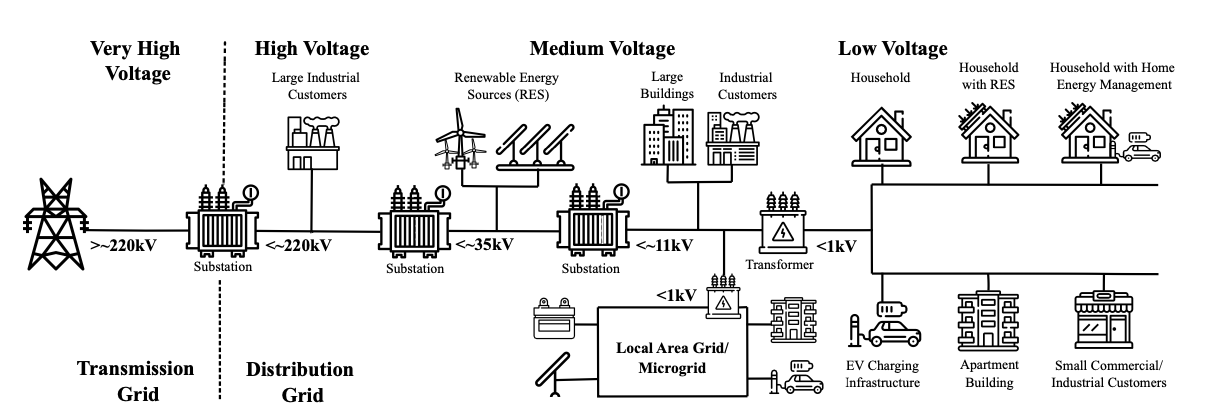
\includegraphics[width=\textwidth]{images/electricity_network.png}
    \caption{Electricity grid \cite{haben2021review}}
    \label{electricity_network}
\end{figure}


\section{Electricity markets}
Electricity markets have gone rapid changes all over the world during the last three decades.
Before this revolution, the power sector was a natural monopoly. In particular, it was characterized by a high vertical integration and by very little market competition. Better technologies in both transmission, generation and distribution are the reasons for such liberal shift. The rationale is simple, a competitive market promotes efficiency and stimulates technical innovation more than a monopoly does.
\\
During the nineties various wholesale electricity markets were established; for example in Chile, Great Britain, the scandinivian block, Australia, New Zealand, the US and Canada. Consequently, new participants, each with a specific task, entered the power market scenario.
\begin{itemize}
    \item Electricity generators produce electricity to be consumed.
    \item Electricity transmission owners 
    move high voltage electricity to electric utility companies whilst ensuring safe and reliable supply.
    \item Electricity grid operators are responsible for scheduling electricity over the transmission network in order to ensure supply demand balance.
    \item Electric utilities deliver power over local lines to consumers. 
    \item Retail energy suppliers purchase electricity in the wholesale market from electricity generators and resell it to consumers.
\end{itemize}
Notice, these functions are not mutually exclusive; that is an entity can provide one or more of these services.


\subsection{The marketplace}
We can differentiate between two kinds of electricity markets: power pools and power exchanges. In power pools, generators bid the prices at which they are willing to produce at different volumes. Then, the market clearing price (MCP) is determined by intersecting the aggregated supply curve and the estimated demand, left panel figure \ref{fig:pool_vs_echange}. Power pools are created on public initiatives of governments. Conversely, power exchanges are created through private agreements between generators, distributors and traders. This is the model followed by most of european countries.
The MCP in power exchanges is determined by the intersection of the aggregate supply curve and the aggregate demand curve, right panel figure \ref{fig:pool_vs_echange}.
\\
It is worth to mention the two biggest power exchanges: Epex and NordPool. Epex operates throughout continental europe. NordPool covers the nordinc and baltic contries.
\\
Moreover, we can differentiate between two popular types of auctions: uniform-price/marginal and pay as bid/discriminatory. Within the uniform price setting, suppliers offering less than the clearing price are paid that price. Analogously, consumers bidding more than the clearing price pay that price. On the other hand, in pay as bid auctions, suppliers are paid the exact price they bid for.


\begin{figure}[!h]
    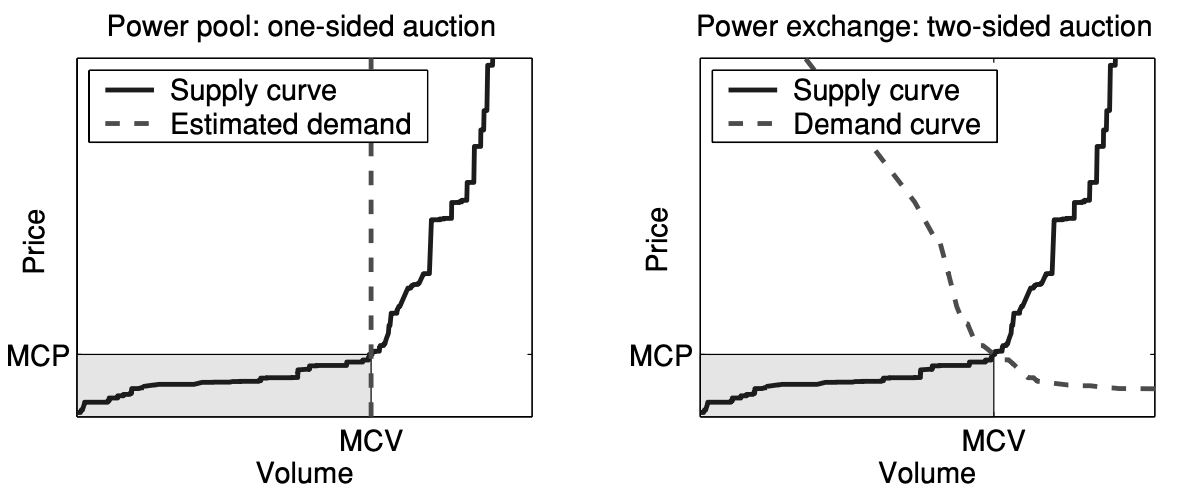
\includegraphics[width=\textwidth]{images/pool_vs_echange.png}
    \caption{Pool market versus power echange \cite{weron2006modeling}}
    \label{fig:pool_vs_echange}
\end{figure}

\subsection{How auctions work}
We can drill down on the auction types, the two most popular forms are day ahead and intraday auctions.
% https://medium.com/@brandonvar/day-ahead-and-intraday-electricity-markets-1eb121dcab47

% \subsection{Day ahead}
The day ahead market is based on a blind auction taking place every day of the year.
During these auctions, the prices of all hours for the next day are traded.
Market participants can enter their buy and sell orders until order book closure, which takes place at 12.00 PM. After that, the market establishes hourly prices by intersecting the demand and supply curves for each hour of the following day.

% \subsection{Intraday}
The intraday market consists of continous trading 24/7. A trade is executed as soon as a buy and a sell order mathch. Electricity can be traded an hour, half-hour, quarter or also 5 minutes before delivery. This enables market participants to balance their positions in real time, should they need to do so.

\subsection{Price peaks}
Electricity market are characterized by spikes in their spot prices; when this happens, the system price jumps abruptly and then drops back within a very short period.
This spikness follows from the non storability of electricity; that is, electricity has to be consumed as it is produced. Therefore, extreme load fluctuations combined with generation outages or transmission failures can result in price spikes.

% outages=interruzione
\subsection{Negative prices}
It is not unusual to observe negative prices in electricity markets, even though they are rare.
The causes of negative prices are inflexible power generation plants and low demand. With inflexibility, it is mean the fact that power sources cannot be switched off and restarted quickly and efficiently.
Thus, producers are faced with the decision of either stopping and restarting their power plant or selling their energy for a negative price; that is they pay consumers for consuming their energy.

\subsection{Nodal and zonal pricing}
Grid configuration and physical limits on electricity lines may lead to congestion. Local marginal price (LMP) and zonal market clearing pricing (ZMCP) are two types of pricing schemes utilized to handle it. The former is adopted in EU contries while the latter is used in the US, figure \ref{fig:eu_zonal} and figure \ref{fig:us_local}.
With zonal market clearing pricing, prices may differ between zones but are the same within the same area.
On the other hand, local marginal price is made up by summing the transmission congestion cost, generation marginal cost and the cost of marginal losses at different buses; buses is where a electicity line or several lines are connected.
\begin{figure}[!h]
    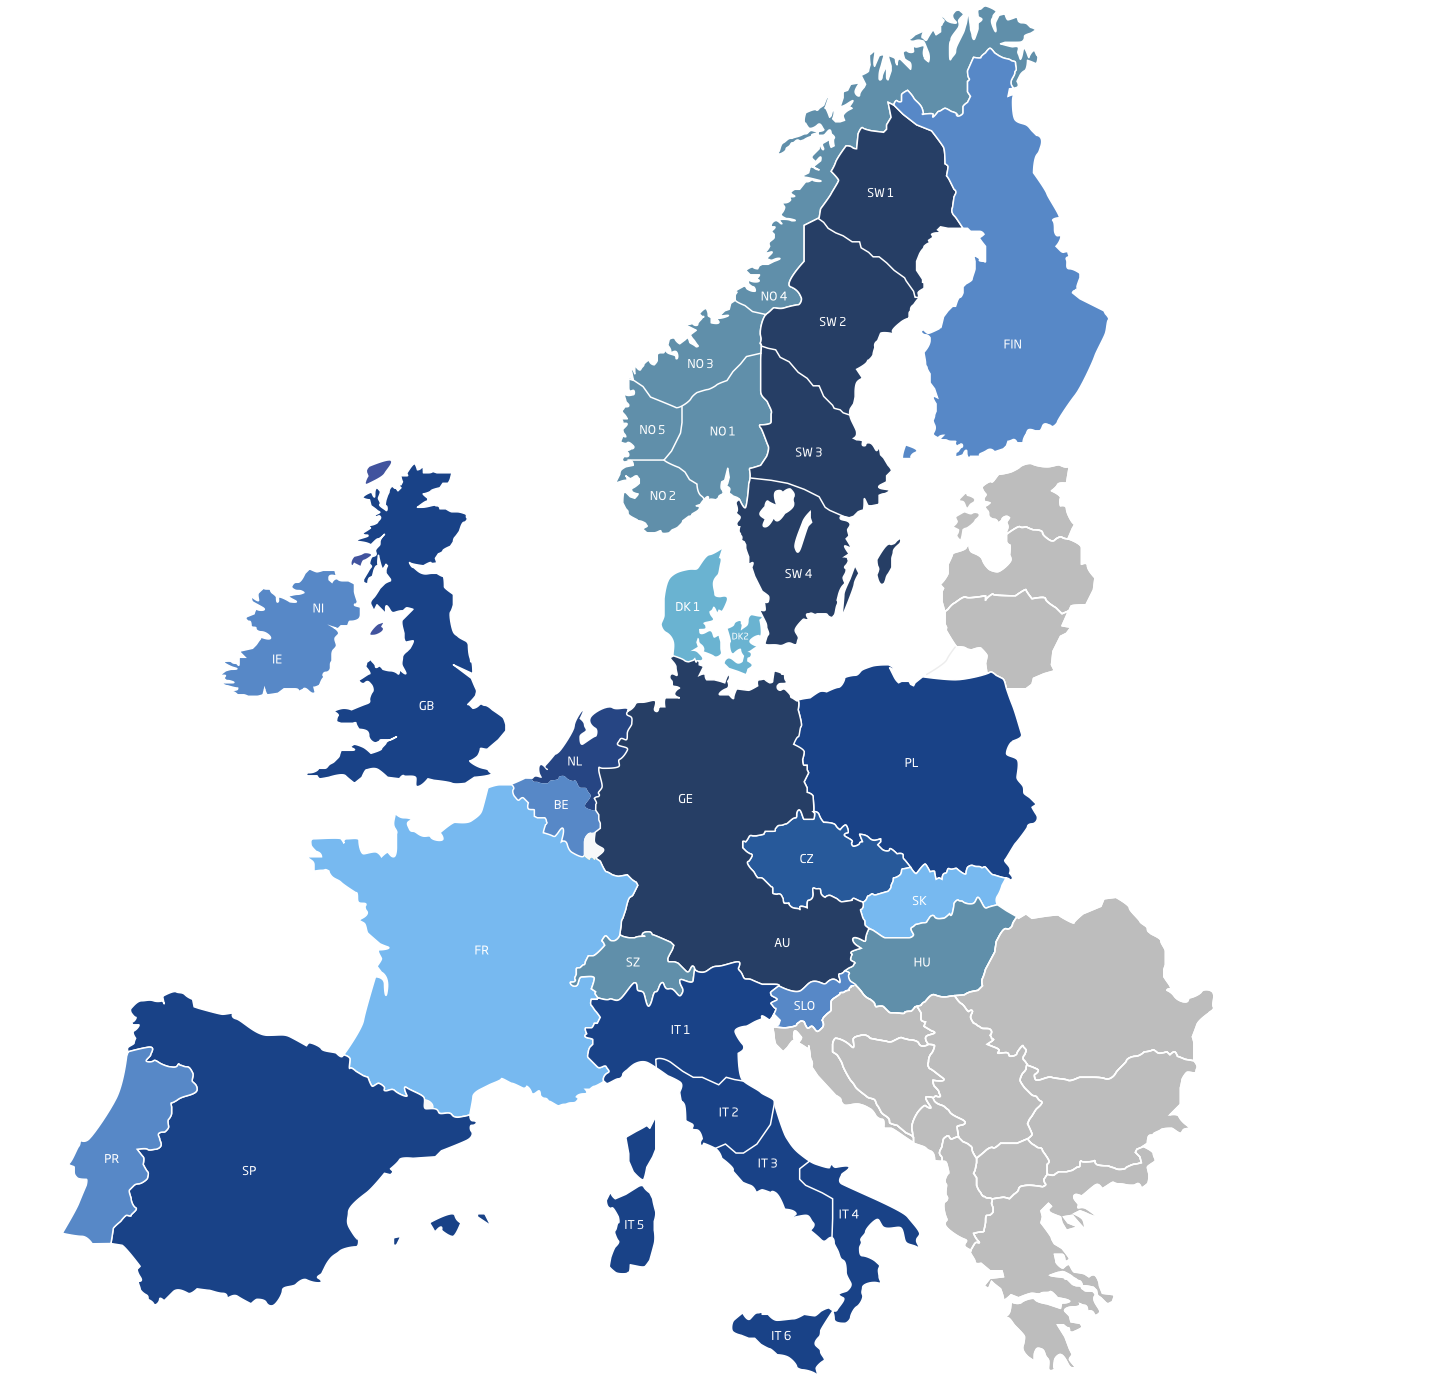
\includegraphics[width=\textwidth]{images/eu_zonal.png}
    \caption{Zonal pricing EU \cite{eu_zonal}}
    \label{fig:eu_zonal}
\end{figure}

\begin{figure}[!h]
    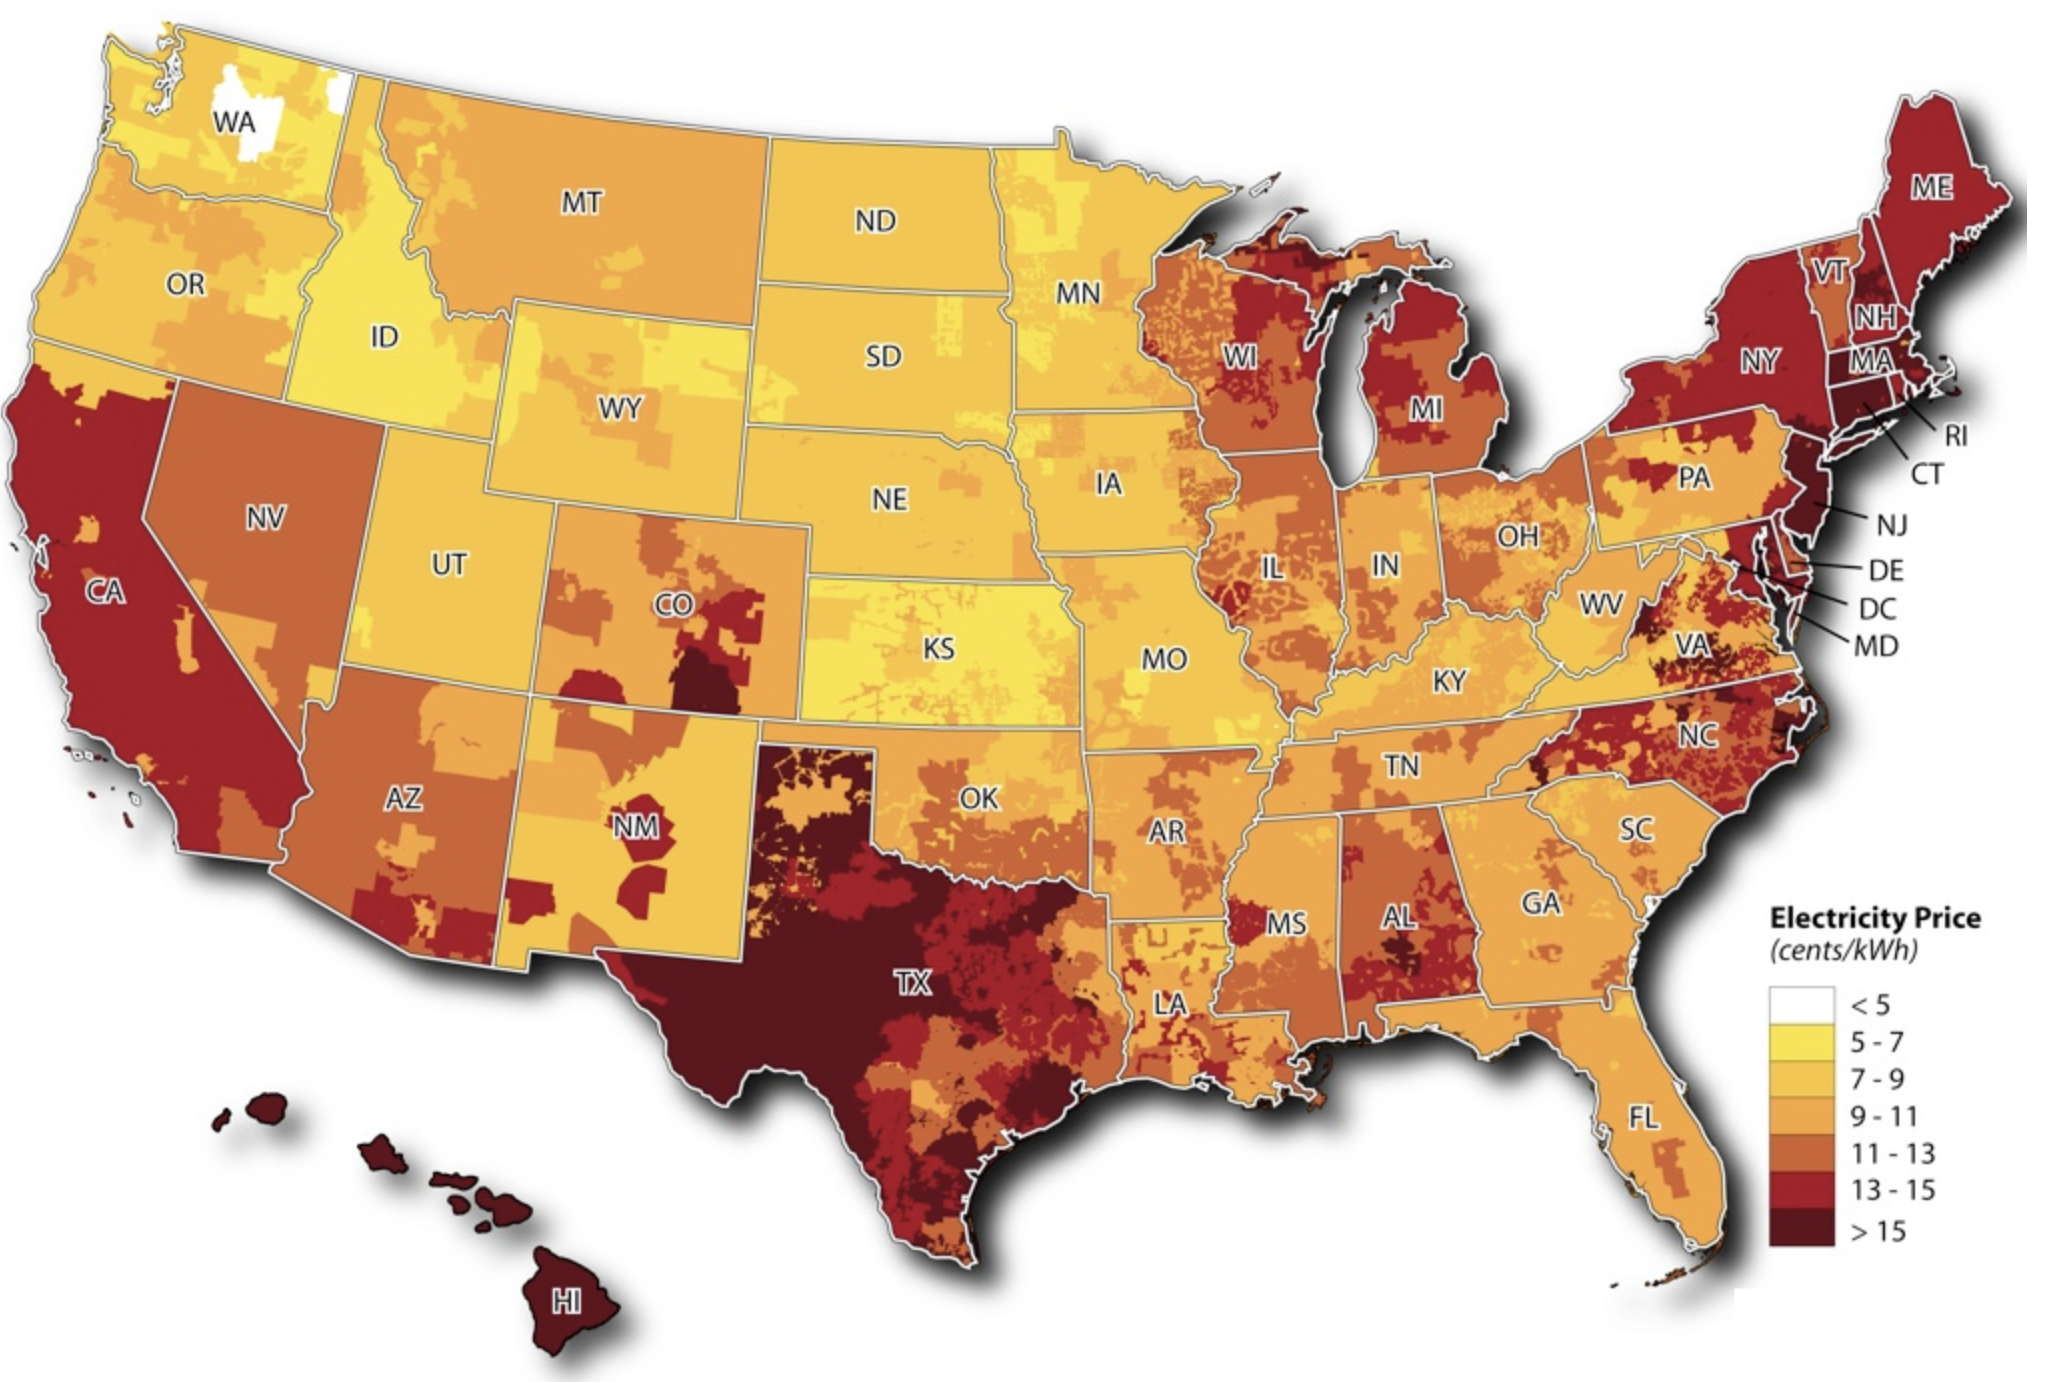
\includegraphics[width=\textwidth]{images/us_local.png}
    \caption{Local pricing US \cite{us_local}}
    \label{fig:us_local}
\end{figure}

% pensodino \subsection{Nodal and Zonal Pricing}
\section{Smart grids}
A smart meter is a digital device recording energy consumption in real time and communicating this data to the supplier and the consumer.
Deployment of smart grids and the digitalisation of the electricity network are intended to increase the energy efficiency of our networks.
The reason is that, smart metering and the electricity network digitalisation  will enable system operators to better monitor the network, plan their investments and manage infrastructure. 
All of this motivates for the need of efficient and robust tools to analyze the vast data resulting from the digitalisation of the power sector.

\section{Renewables}
% https://www.pnnl.gov/explainer-articles/renewable-integration
A pressing challenge facing policymakers today is the energy transition towards cleaner energy, see figure \ref{fig:electricity_production_by_source} for an up to date breakdown on energy production by source. Such move is intended to mitigate the effects of climate change and reduce pollution at the same time.
This transition passes through renewables integration into the electric grid. 
Nevertheless, integrating renewables into the existing electric grid involves several technical challenges. First, we need to develop infrastructures and technologies capable of connecting renewable power plants with the existing grid. For example, connecting renewables power plants located in remote and offshore locations to high voltage powerlines is not trivial.
Additionally, renewables such as wind and solar are characterized by seasonalities and depend heavily on weather conditions. Therefore, balancing the electricity network and mantaining stability will become harder for grid operators; they will need more flexibility in the grid and develop new approaches in order to achieve their goals.

\begin{figure}[!h]
    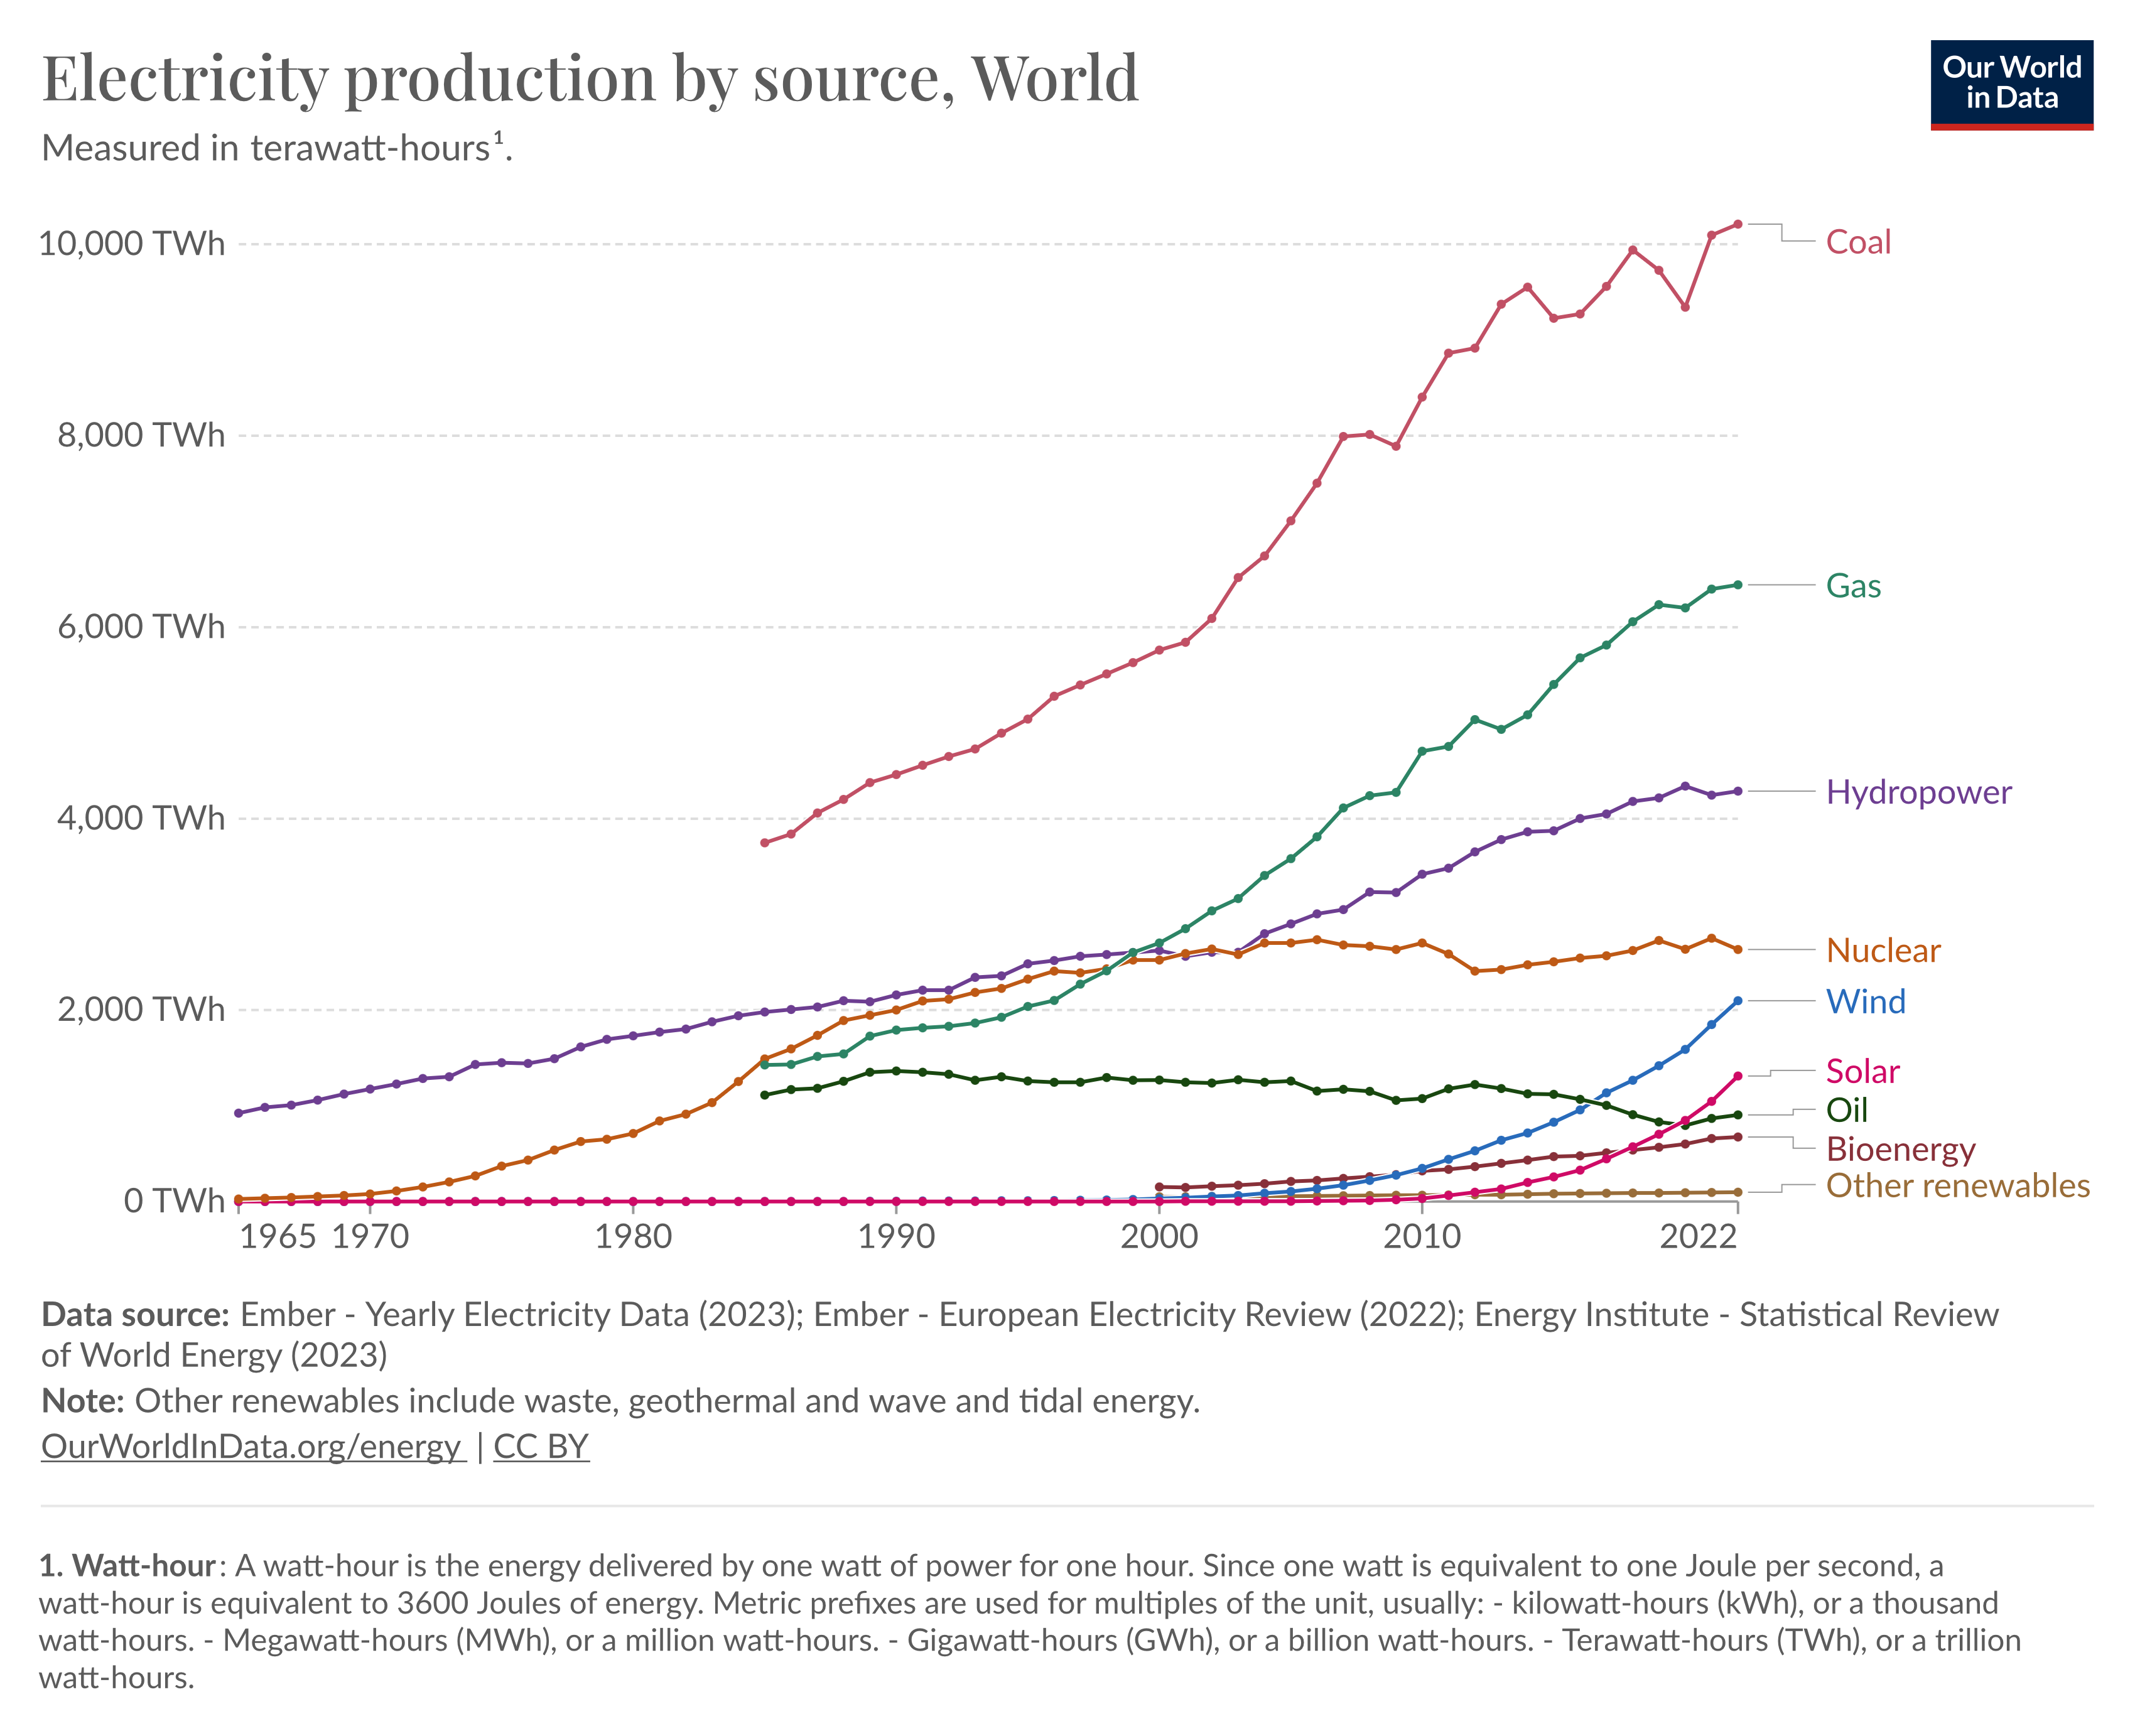
\includegraphics[width=\textwidth]{images/electricity-production-by-source.png}
    \caption{Electricity production by source}    
    \label{fig:electricity_production_by_source}
\end{figure}



\chapter{Evaluation metrics}\label{metrics}
Proper evaluation methods guide researchers in choosing the model that best fits their needs. This chapter is dedicated to the most common evaluation metrics adopted by academics in the field of electricity forecasting. Error metrics and measures vary depending on whether we are concerned with point or probabilistic forecasts. Additionally, note that the latter can take different forms which therefore requires different measures.
\section{Mean absolute error}\label{mae}
Consider the time series with actual values given by $y=(y_{n+1}, y_{n+2},\dots, y_{n+h})$
and its $h$ step ahead point forecast $\hat{y}=(\hat{y}_{n+1}, \hat{y}_{n+2},\dots, \hat{y}_{n+h})$ the mean absolute error (MAE) is defined as
\begin{definition}
    The mean absolute error is defined as
    $$
    \mathrm{MAE}(y,\hat{y})=\frac{1}{h}\| y- \hat{y}\|_{1}=\frac{1}{h}\sum\limits_{k=1}^{h}|y_{n+k}-\hat{y}_{n+k}|
    $$
\end{definition}

\section{Root mean squared error}\label{rmse}
\begin{definition}
    The root mean squared error is defined as
    $$
    \mathrm{RMSE}(y, \hat{y})=\frac{1}{\sqrt{h}}\|y-\hat{y}\|_{2}=\sqrt{\frac{\sum\limits_{k=1}^{h}(y_{n+k}- \hat{y}_{n+k})^2}{h}}
    $$
\end{definition}

Mean absolute error and root mean squared error posses the useful property of being expressed in the same units of the data, thus enabling meaningful comparisons.
However, a drawback of such measures is that we cannot use them to compare accuracy between time series which have different magnitudes. For instance, a day ahead error of 1kWh is negligible when considering a daily demand of 100kWh while the same error is considerably big when daily demand is 2kWh. This consideration leads to relative accuracy scores. Between those the mean absolute percentage error (MAPE) is by far the most popular.


\section{Mean absolute percentage error}\label{mape}. 
\begin{definition}
    The mean absolute percentage error is defined as
    $$
    \mathrm{MAPE}(y,\hat{y})=\frac{100}{h}\sum\limits_{k=1}^{h}\frac{|y_{n+k}-\hat{y}_{n+k}|}{|y_{n+k}|}$$
\end{definition}

\section{Root mean squared percentage error}\label{rmspe}
\begin{definition}
    The root mean squared percentage error is defined as
    $$
    \mathrm{RMSPE}(y,\hat{y})=100\cdot\sqrt{\frac{1}{h}\sum\limits_{k=1}^{h} \left(\frac{|y_{n+k}-\hat{y}_{n+k}|}{|y_{n+k}|}\right)^2}
    $$
\end{definition}
Mean absolute percentage error and root mean squared percentage error may not be appropriate for series which have zero or very small values, for example, electricity demand at the household level. The result is a large score regardless of the absolute errors.
Scaled errors constitute a robust family of scores.
\section{Mean absolute scaled error}\label{mase}
\begin{definition}
    The mean absolute scaled error is defined as
    $$
    \mathrm{MASE}(y,\hat{y})=\frac{1}{h}\sum\limits_{k=1}^N\frac{|y_{n+k}-\hat{y}_{n+k}|}{\frac{1}{h-1}\sum\limits_{k=2}^{h}|y_{k}-y_{k-1}|}
    $$
\end{definition}
In the denominator we have the error of the naïve/persistence model. 
In this model, the current demand makes up the prediction for the next time step, that is $\hat{y}^{\mathrm{naive}}_{n+1}=y_{n}$.
\section{Root mean squared scaled error}\label{rmsse}
\begin{definition}
    The root mean squared scaled error is defined as
    $$
    \mathrm{RMSSE}(y,\hat{y})=\sqrt{\frac{1}{h}\sum\limits_{k=1}^N\left(\frac{|y_{n+k}-\hat{y}_{n+k}|}{\frac{1}{h-1}\sum\limits_{k=2}^{h}|y_{k}-y_{k-1}|}\right)^2}
    $$
\end{definition}


\section{Pinball score}\label{pinball}
The pinball score or quantile score is used to measure the accuracy of a quantile forecast.
\begin{definition}
    The pinball loss is defined as
    $$
    \mathrm{Pinball}(y_{t},\hat{y}_{t,q},q)=
\begin{cases}
(q-1)(\hat{y}_{t,q}-y_{t}) & y_t > \hat{y}_{t,q} \\
q(\hat{y}_{t,q}-y_t) & y_t \leq \hat{y}_{t,q}
\end{cases}
$$
\end{definition}
The pinball loss is an asymmetric function, it weights its score differently depending on the error sign and on the quantile considered, see Figure \ref{fig:pinball}.
\begin{figure}
    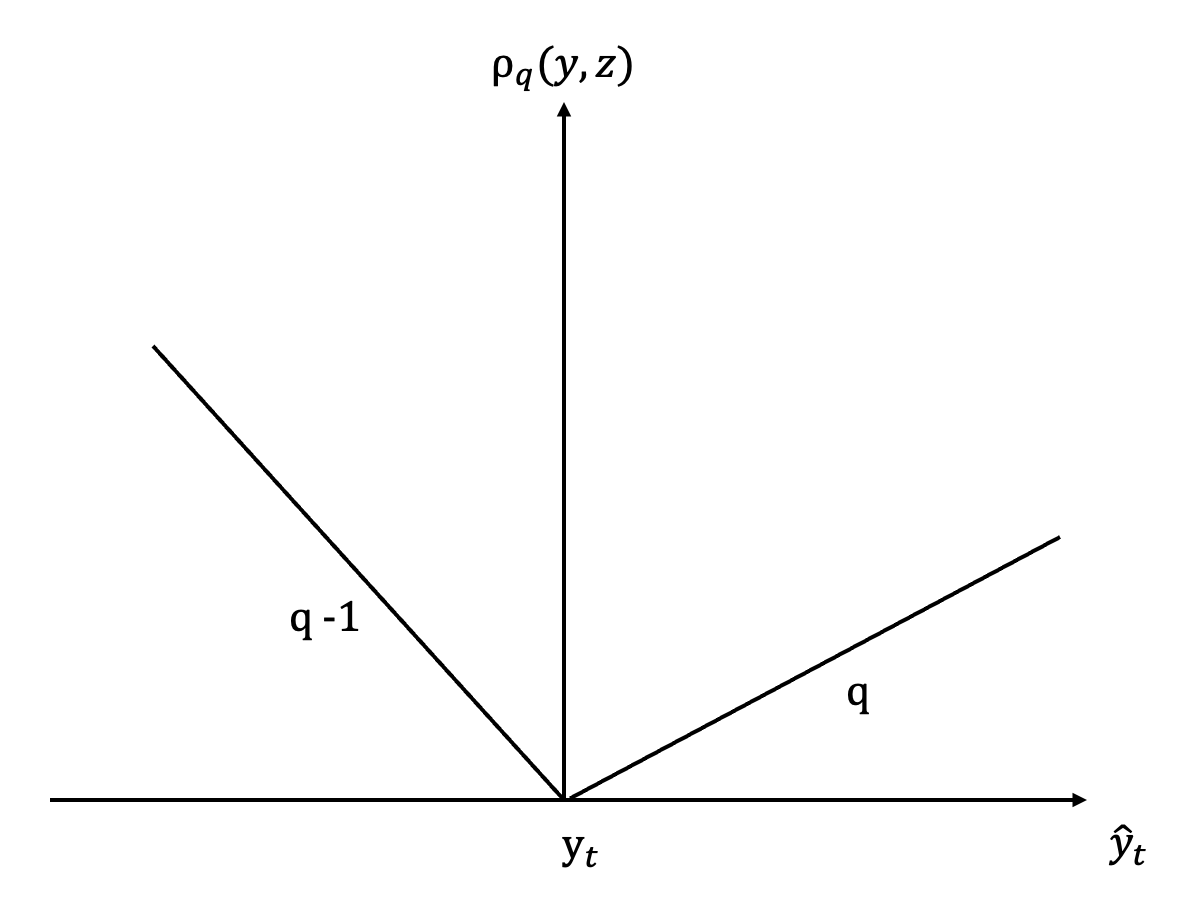
\includegraphics[width=\textwidth]{images/pinball_loss.png}
    \caption{Pinball loss}
    \label{fig:pinball}
  \end{figure}
By averaging all the pinball losses over all quantiles and over the whole forecast horizon, we obtain the pinball loss of the probabilistic forecast.
\section{Winkler score}
\begin{definition}
    The Winkler score is defined as
    $$
    \mathrm{Winkler}(y_t,  u_{t},l_{t},q)=\begin{cases}
        \delta & l_{t}\leq y_{t}\leq u_{t}\\
        \delta+2(l_{t}-y_{t})/\alpha & y_{t}< l_{t}\\
        \delta+2(l_{t}-u_{t})/\alpha & y_{t} \geq u_{t}
    \end{cases}
    $$
\end{definition}
Where $\delta$ is the prediction interval (PI) width, that is $\delta=u_t-l_t$, $u_t$ is the prediction interval upper threshold and $l_t$ is the prediction interval lower threshold at time step $t$. This score penalizes observations falling outside the prediction interval and rewards narrow prediction intervals.
\section{Continous ranked probability score}
The continous ranked probability score (CRPS) measures the difference between the estimated cumulative distribution $\hat{F}$ and the empirical cumulative density function (CDF).
\begin{definition}\label{def_crps}
    The continous ranked probability score is defined as
    $$
    \mathrm{CRPS}(y, \hat{F})=\int\limits_{-\infty}^{\infty}\left(\hat{F}(x)-\mathbb{I}_{\{x-y\}} \right)^2 dx
    $$
\end{definition}
% Nevertheless, we can evaluate the integral in closed form. 
Where the indicator function is defined as 
    $$\mathbb{I}_{\{z\}}=
\begin{cases}
0, & z<0\\
1, & z \geq 0
\end{cases}$$
\\
For a visualisation see Figure \ref{fig:crps}. The grey area is what contributes toward the CRPS score.
The better the estimated cumulative density function is the smaller the total CRPS score will be.
\begin{figure}
    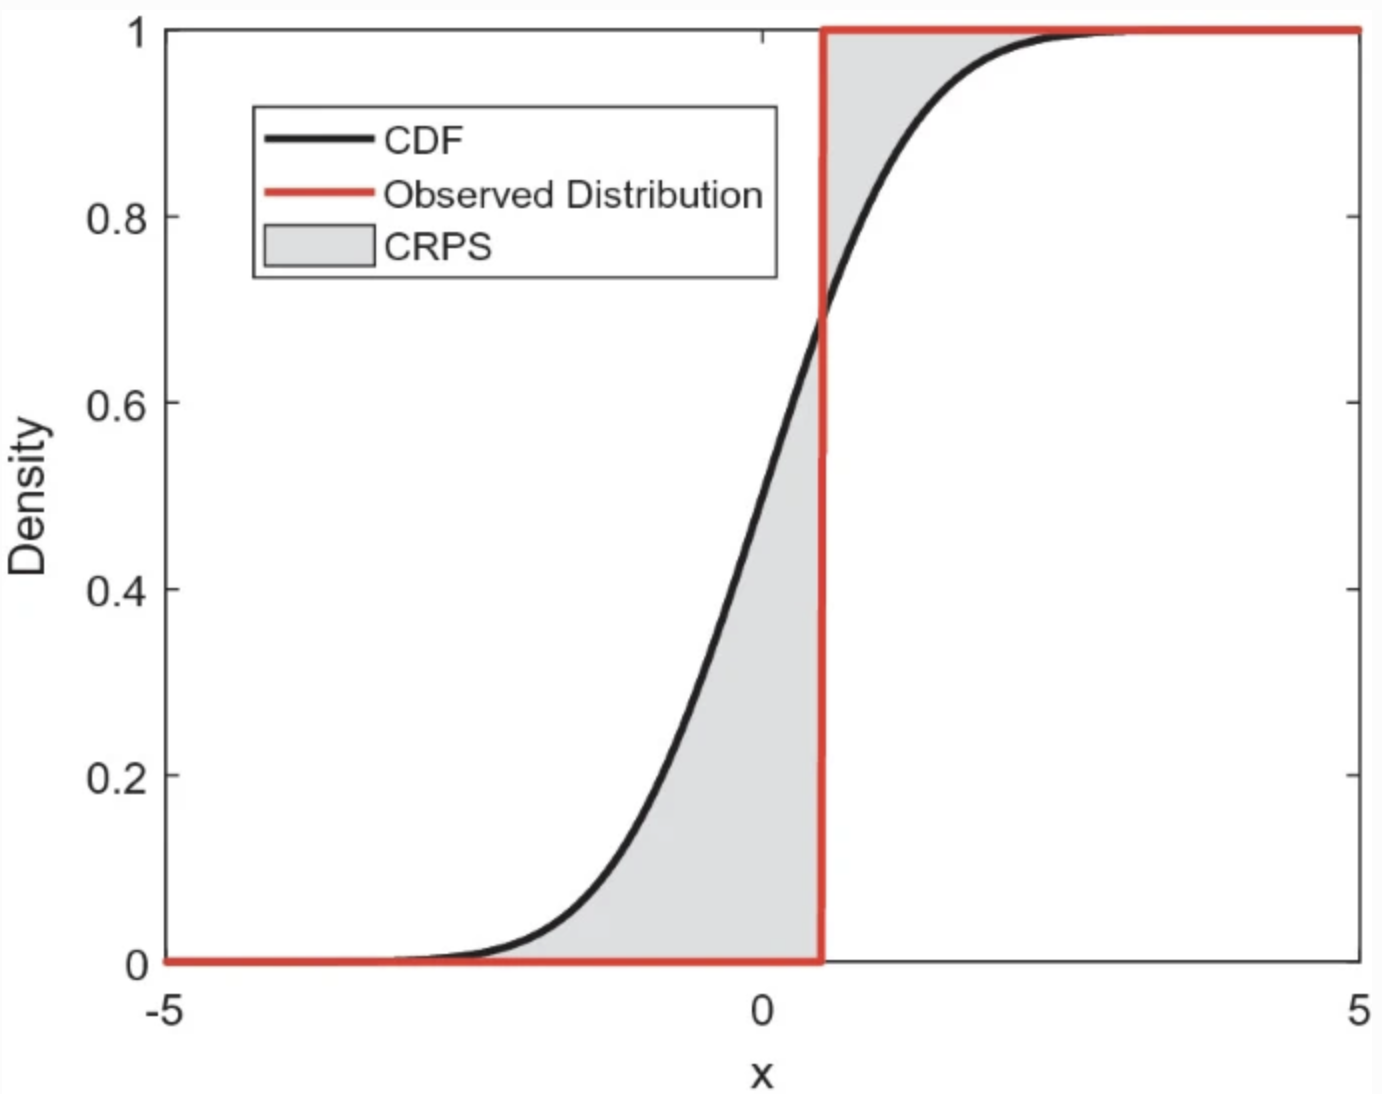
\includegraphics[width=\textwidth]{images/crps.png}
    \caption{CRPS integral \cite{haben2023core}}
    \label{fig:crps}
  \end{figure}
  \\
It is worth noting, that the CRPS integral can be rewritten in terms of expectations. This makes its evaluation easier, since we know that the sample mean converges to the expectation for sufficiently big sample sizes by the law of large numbers. This was first pointed out by \cite{proper_scores}, where the authors take advantage of Lemma 2.2 of \cite{new_multi_test2} or equivalently identity (17) of \cite{new_multi_tes1}.
\\
\begin{lemma}
    Let $X_1$, $X_2$, $Y_1$, $Y_2$ be independent real random variables with finite expectations. Let $X_1,X_2$ be identically distributed with distribution function $F$ and let $Y_1,Y_2$ be identically distributed with distribution function $G$. Then
   \begin{equation}\label{eq:crps_expectation}
    \mathbb{E}(|X_1-Y_1|)-\frac{1}{2}\mathbb{E}(|X_1-X_2|)-\frac{1}{2}\mathbb{E}(|Y_1-Y_2|)=\int\limits_{-\infty}^{\infty}\left(F(x)-G(x)\right)^2dx
\end{equation}
\end{lemma}
Notice that, in our case, Equation \ref{eq:crps_expectation}, the distribution $G$ of $Y_1$ and $Y_2$ is degenerate, with all probability mass on a single point $y$.
%  (x notation will need to be cleaned here). Since $G(t)=:$
It follows that the third addend in the summation is zero. That is because $Y_1$ and $Y_2$ both following distribution $G$ implies that $\mathbb{E}(|Y_1-Y_2|)$ corresponds to the difference of two equal constant numbers.
\\
Additionally, since $Y_1$ is just a constant, we have $Y_1=y$.
\\
Putting everything together we have obtained an alternative way of computing the CRPS score.
\begin{equation}
    \int\limits_{-\infty}^{\infty}\left(\hat{F}(x)-\mathbb{I}_{\{x-y\}} \right)^2 dx=\mathbb{E}(|X_1-y|)-\frac{1}{2}\mathbb{E}(|X_1-X_2|)
\end{equation}
\\
\section{Probability integral transform}
The probability integral transform (PIT) is a method to assess visually the quality of a probabilistic forecast. PIT is obtained by applying the predicted cumulative density function $\hat{F}$ to the data. If applying such CDF to the data results in a uniform distributed PIT, then $\hat{F}$ is a valid prediction. If not, $\hat{F}$ is not a good estimate of the CDF for the considered data. Figure \ref{fig:pit} provides an example, applying the true CDF results in a well calibrated PIT (left). Alternatively, applying a bad CDF results in either an overdispersed (middle) or underdispersed (right) PIT.
\begin{figure}
    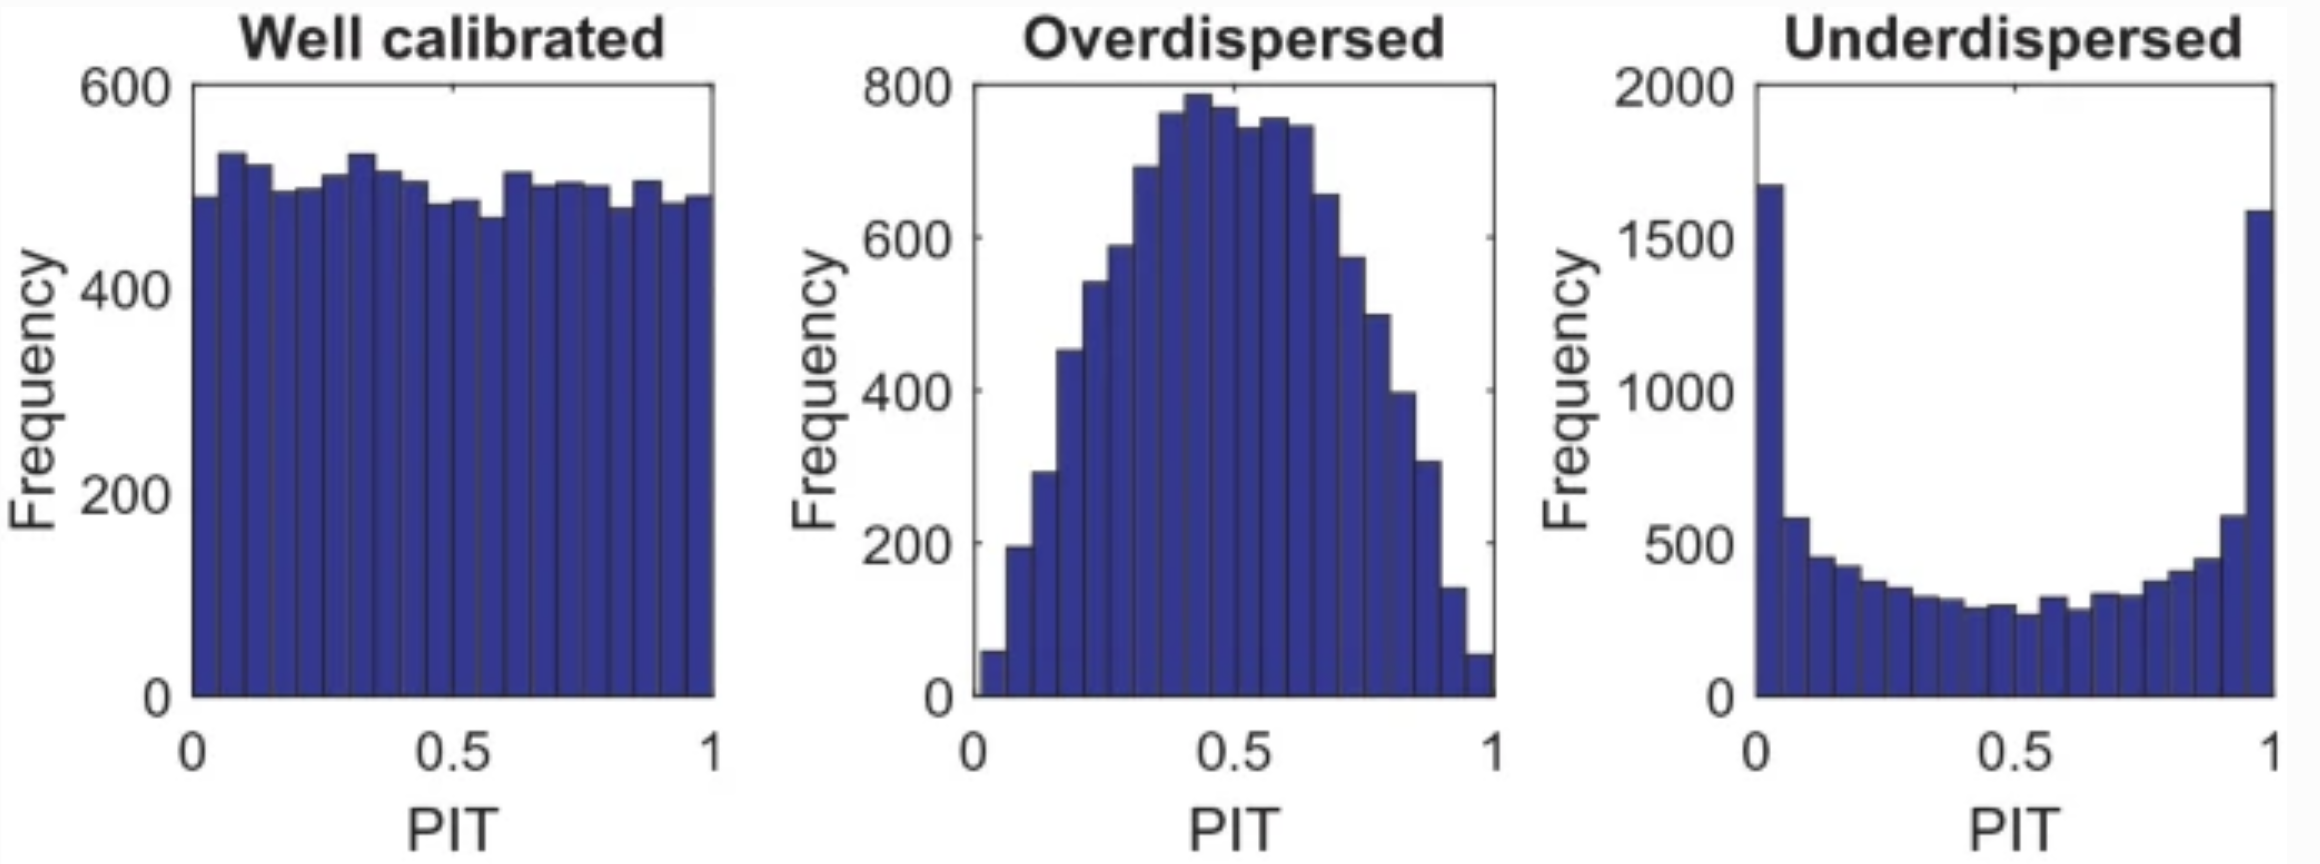
\includegraphics[width=\textwidth]{images/pit.png}
    \caption{Probability integral transform types \cite{haben2023core}}
    \label{fig:pit}
  \end{figure}
\\
%RELIABILITY PLOT
%PICP,NMPIW,CWC,unconditional coverage(arora)-->Probability density forecasting of wind speed based on quantile regression and kernel density estimation Lei Zhang

% Reliability and sharpness \section{Criteria}-->Recent advances in electricity price forecsating a review of probabilistic forecasting Weron
% Two criteria are used in literature to evaluate probabilistic forecasting: sharpness and reliability. Reliability means 

\chapter{Exploratory Analysis and Data ETL}\label{eda}
- Explain how data has been retrieved.

- Data provider EPEX(entsoe retrieves its data)

- Explain the ETL(Extract Transform Load) pipeline
I set up.

- Explore data in order to get useful insights for
how to tune the models to get the most of them.

- correlation between temperatures and load

- Correlation and auto correlation plots

- Split train and test dataset
Explain carefully why it is important to carry
out an out of sample test and not in sample.
In sample test involves look ahead bias because we are
fitting the model on the data we want to predict,
thus it overfits on the data considered but it does
not generalize well.


This section covers the datasets used in our experiments, attributes and features will be thoroughly described.
Next, we will explain the ETL pipeline that we set up in order to ease the workflow of our comparison studies.
Finally, in order to to bettern understand patters within the data, we carry out an exploratory data analysis.

\section{Dataset}
The chosen datasets for probabilistic load forecasting, were the data from the GEFCom 2014 competition. The data is freely hosted on Dr. Hong blog \cite{hong2016probabilistic}.
The main reason was that, these dataset are considered an a excellent test case for comparing predictive models between the EF community. Additionally, the scores of the competing models are freely available, this enables us to carry out a clean and transparent comparative study.
The GEFCom 2014 consisted of four tracks: price, load, wind power and solar power forecasting. 
The GEFCom2014 folder contains a zip file for each of the four tracks.
This thesis work is focuesed on providing forecasts for the load and price quantities.
\\
\subsection{Price track}
In the price forecasting track, the goal was to predict the electricity price for the next 24 hours of a single zone. 
The data can be found in the GEFCom2014-P\_V2 zip file alongside a set of instructions and the benchmark forecasts.
This data consisted of time series for the locational marginal price, for the zonal load and for the system load. The data covers the time interval ranging from the 1st of January 2011 to the 15th of June 2013, see figure \ref{fig:price_track_fig1}. 
Additionally, as the competition went on, the real observed data of the previous tasks were made available.
The fifteen target days ordered by task number are: 16/06/2013, 17/06/2013, 24/06/2013, 04/07/2013, 09/07/2013, 13/07/2013, 16/07/2013, 18/07/2013, 19/07/2013, 20/07/2013, 24/07/2013, 25/07/2013, 07/12/2013, 08/12/2013. 
\begin{figure}[!h]
    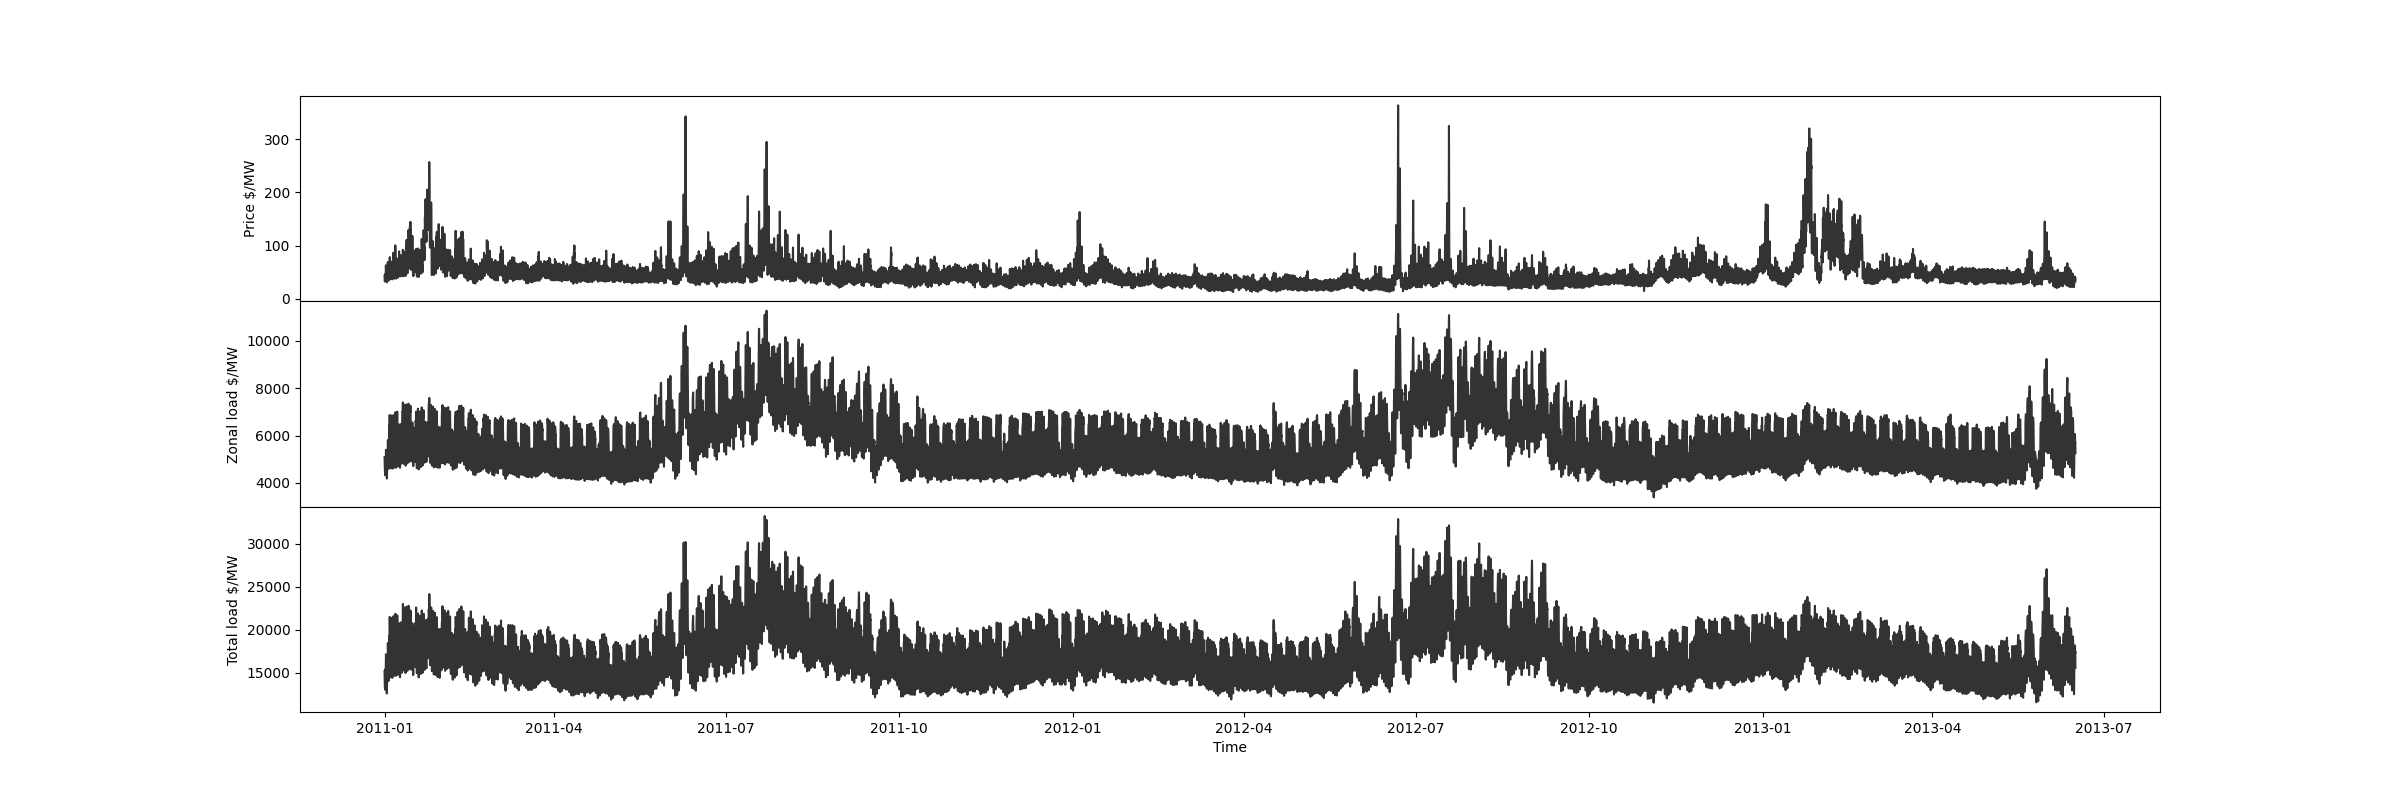
\includegraphics[width=\textwidth]{images/price_track_fig1.png}
    \caption{Price track}
    \label{fig:price_track_fig1}
\end{figure}
\subsection{Load track}
In the load track, contestant were asked to provide one month ahead hourly probabilistic forecasts on a rolling basis for 15 consecutive rounds. To get started, in the first round, organizers provided 69 months of hourly load data (from 01/01/2005 to 30/10/2010) and 117 months of hourly temperature data (from 01/01/2001 to 30/10/2010). 
As for the price track, the true observed data from the previous track were made available as the competition progressed.
\\
The data for load forecasting is contained in the GEFCom2014-L\_V2 zip file. Within this subfolder, we a txt with the competition instructions and 15 folders one for each of the consecutive tasks. For each of those we have the prediction of the competition benchmark model and the train file upon which we will fit our model.
Each data from the various task folders are shifted by one months between others.
\\
In order to compare our model performance with the winning entries of the GEFCom2014 load competition, we will refer to the Provisional\_Leaderboard\_V2 file contained also in the GEFCom2014 Data directory.
% Notice a quick premise, within this xsls file the authors opted for various scores to compare the entries performance. This choice was motivated by the need 
% to give a proportial weight to each task when averaging between them; that is in order to not penalise too much the tasks with higher point spreads. Furthermore, additional factors such as frequency of benchmark outperformance, and robustness and clarity in methodology explaination.
\\
Notice, the pinball scores for the load track are stored inside the subtab L-score-0/L-score-2 of Provisional\_Leaderboard\_V2.

\section{ETL}


\section{EDA}

\chapter{Implementation}\label{implementation}
This section is intended to explain and aid for reproducibility studies. Hereafter, the specific libraries used and the custom implementations are thoroughly documented.

For the list of Python packages needed, see the requirement.txt file on the \href{https://github.com/luca-pernigo/ThesisKernelMethods}{github repo}.
% - indicate computer specifics
All experiments have been carried out on a 3.2 GHz 16GB Apple M1 Pro.


% Section documenting code

% - Explain how methods' implementation has been
% adapted to my specific setting.

% - Explain in detail how to my src code has been implemented
% its rationale and how to use it.

% - As I explain code scripts go over the test, to 
% explain better my ideas.

% - Indicate also hyperparameters maybe in each subsection

\section{Point forecasting}
\subsection{Multiple linear regression}
For multiple linear regression the one from the \href{https://scikit-learn.org/stable/}{sklearn} library has been used.

\subsection{Trigonometric seasonality Box-Cox transformation AR\-MA errors trend and seasonal components}
The Tbats implementation is available at \href{https://github.com/intive-DataScience/tbats}{https://github.com/intive-Data-Science/tbatsx}.
In our application we specified as hyperparameters the length of seasons, that is, 24 for the daily seasonality and 168 for the weekly seasonality.

\subsection{Prophet}
The \href{https://facebook.github.io/prophet/docs/quick_start.html}{prophet} model has been applied by employing the Python API provided by Meta.

\subsection{K-nearest neighbours}
The object KNeighborsRegressor of the \href{https://scikit-learn.org/stable/}{sklearn} module neighbors has been used with 12 neighbours and the Euclidean distance.

\subsection{Support vector regression}
The object SVR of the \href{https://scikit-learn.org/stable/}{sklearn} module svm has been used by specifying the linear kernel.

\subsection{Long short term memory}
The LSTM predictor has been built using the \href{https://pytorch.org}{torch} library, see Section \ref{sec:lstm point} for architecture details.

\subsection{Kernel ridge regression}
The object KernelRidge of the \href{https://scikit-learn.org/stable/}{sklearn} module kernel\_ridge has been used with the Gaussian RBF kernel.

\subsection{Kernel support vector regression}
The object SVR of the \href{https://scikit-learn.org/stable/}{sklearn} module svm has been used with the Gaussian RBF kernel.
% by specifying rbf as the kernel parameter.

\section{Probabilistic forecasting}
\subsection{Linear quantile regression}
The implementation of \href{https://www.statsmodels.org/dev/generated/statsmodels.regression.quantile_regression.QuantReg.html}{quantile\_regression.QuantReg} from the regression module of statsmodels has been used.
The model is fitted through iterative reweighted least squares.
\subsection{Quantile gradient boosting machine}
The implementation of \href{https://scikit-learn.org/stable/modules/generated/sklearn.ensemble.GradientBoostingRegressor.html}{GradientBoostingRegressor} from the sklearn.ensemble submodule has been used.
\subsection{Quantile forest}
The implementation of \href{https://pypi.org/project/quantile-forest/}{quantile\_forest.RandomForestQuantileRegressor} has been used. This estimator is compatible with scikit-learn API \cite{Johnson2024}.
\subsection{Kernel quantile regression}
Kernel quantile regression had no previously implemented Python open source library, thus, the need of implementing our own version.
\\
The scikit-learn team provides a project template for the creation of estimators compatible with scikit-learn functionalities. Therefore, the KQR class is derived from the scikit-learn BaseEstimator and the mixin class RegressorMixin.
Our KQR class is initialised by providing a quantile, the regularisation term $C$, the kernel family and its corresponding hyperparameters.
\\
In the fit method, we set up and solve the convex optimisation problem through the interior point algorithm. This algorithm is taken from the cvxopt library, see its official manual \citeW{vandenberghe2010cvxopt} for a reference.
When using this library, it is important to keep two things in mind. First this library assumes the quadratic term of the optimisation problem to be multiplied by the 0.5 factor, thus, we just have to provide the $Q$ matrix with no 0.5 in front.
Secondly, in order to specify multiple inequalities we have to stack them and provide them as a single matrix.
\\
Once a solution to the convex problem has been found, we create a mask for the support vectors of the estimator in order to estimate the constant term of our kernel quantile regressor.
\\
In the predict method, we pass a matrix $X\_eval$ of independent variables, next we compute the kernel matrix between $X\_train$ and $X\_eval$ and obtain $y\_eval$ with the formula $y=\alpha^\intercal K+b$.
\\
This estimator is compatible with in built scikit-learn methods like gridsearch, crossvalidation and scoring rules. Moreover, this code is compatible with sklearn in built kernel functions \href{https://scikit-learn.org/stable/modules/classes.html#module-sklearn.metrics.pairwise}{sklearn.metrics.pairwise} and \href{https://scikit-learn.org/stable/modules/classes.html#module-sklearn.gaussian_process.kernels}{sklearn.gaussian\_process.kernels}. Functions supported by our kernel quantile regression include: Gaussian RBF, Absolute Laplacian, Matern 3/2, Matern 5/2, Linear, Cosine, Sigmoid, Periodic, Polynomial and custom composition of kernels. 
Kernels from these two submodules use a different convention in the hyperparameters. The former has the lengthscale parameter in the numerator while the latter in the denominator. In order to meaningfully compare across different kernels we made them consistent in this aspect. For this purpose we adhere to the convention of having lengthscale hyperparameters in the denominator.

% NOTICE, these kernel implementations differ in the form of passed parameters in the former we pass in the numerator gamma while in the latter we pass l, which stands for length scale in the denominator. To cross validate overt the same range of parameter across the different kernels we made sura that gamma=1/l.


% \\
% Up to now, there are only two open source implementation of the quantile kernel regression. Nevertheless they are both in R, that is there exists no python, matlab or julia open source implementation. 

% Following are reported the results of a comparative study between our own implementation and the one of the R library kernlab


% (i guess it is in C or C++ and then binded to R).
% \subsubsection{Python versus R implementation}
% In this section, a comparison study has been carried out in order to inspect the competitiveness of our implementation with the existing one for the R programming language.

\chapter{Experiments Analysis}\label{experiments}
Analysis of experiments and results
\\
Building on the theory introduced in \ref{ch:point} and \ref{ch:prob}, this section covers the experiments carried out and the results obtained.

- Comments
\\
- Comparison
\\
- Table of loss scores
\\
Plots:
\\
- Plots for visualizing timeseries with quantiles bounds
\\
- Other plots that will come up to mind

\section{Quantile forecasting}
In this subsection we compare performance of quantile regressor considering the GEFCom2014 dataset.
\\
- experiment for quantile estimator on gefcom2014 and we are good



%SYMBOLS LISTINGS

%For mathematical terms \ensuremath
% \glsxtrnewsymbol[description={Autoregressive exogenous model}]{ARX}{\ensuremath{ARX}}

%A
\glsxtrnewsymbol[description={Akaike information criterion}]{AIC}{AIC}
\glsxtrnewsymbol[description={Artificial neural network}]{ANN}{ANN}
\glsxtrnewsymbol[description={Autocorrelation function}]{ACF}{ACF}
\glsxtrnewsymbol[description={Autoregressive model}]{AR}{AR}
\glsxtrnewsymbol[description={Autoregressive moving average model}]{ARMA}{ARMA}
\glsxtrnewsymbol[description={Autoregressive integrated moving average model}]{ARIMA}{ARIMA}
\glsxtrnewsymbol[description={Autoregressive exogenous model}]{ARX}{ARX}

%B
\glsxtrnewsymbol[description={Bayesian information criterion}]{BIC}{BIC}


%C
\glsxtrnewsymbol[description={Computational intelligence}]{CI}{CI}
\glsxtrnewsymbol[description={Conditional kernel density}]{CKD}{CKD}
\glsxtrnewsymbol[description={Continous ranked probability score}]{CRPS}{CRPS}

%D
\glsxtrnewsymbol[description={Distributional neural network}]{DDNN}{DDNN}


%E
\glsxtrnewsymbol[description={Exploratory data analysis}]{EDA}{EDA}
\glsxtrnewsymbol[description={Electricity forecasting}]{EF}{EF}
\glsxtrnewsymbol[description={Electricity load forecasting}]{ELF}{ELF}
\glsxtrnewsymbol[description={Empirical mode decomposition}]{EMD}{EMD}
\glsxtrnewsymbol[description={Electricity load forecasting}]{EPF}{EPF}
\glsxtrnewsymbol[description={Exponential smoothing models}]{ESM}{ESM}
\glsxtrnewsymbol[description={Extract transform load}]{ETL}{ETL}
\glsxtrnewsymbol[description={Electric vehicles}]{EVs}{EVs}

%G
\glsxtrnewsymbol[description={Generalized additive models}]{GAMs}{GAMs}
\glsxtrnewsymbol[description={Gradient boosting regression tree}]{GBRT}{GBRT}
\glsxtrnewsymbol[description={Global energy forecasting competition}]{GEFCom}{GEFCom}
\glsxtrnewsymbol[description={Gaussian process regression}]{GPR}{GPR}


%H
\glsxtrnewsymbol[description={Holt-Winters-Taylor exponential smoothing method}]{HWT}{HWT}

%K
\glsxtrnewsymbol[description={Kernel density estimation}]{KDE}{KDE}


%L
\glsxtrnewsymbol[description={Load marginal price}]{LMP}{LMP}
\glsxtrnewsymbol[description={Long short term memory}]{LSTM}{LSTM}
\glsxtrnewsymbol[description={Low carbon technologies}]{LCTs}{LCTs}
\glsxtrnewsymbol[description={Least squares support vector regression}]{LSSVR}{LSSVR}

\glsxtrnewsymbol[description={Low voltage}]{LV}{LV}

%M
\glsxtrnewsymbol[description={Market clearing price}]{MCP}{MCP}
\glsxtrnewsymbol[description={Market clearing volume}]{MCV}{MCV}
\glsxtrnewsymbol[description={Mean absolute error}]{MAE}{MAE}
\glsxtrnewsymbol[description={Mean absolute scaled error}]{MASE}{MASE}
\glsxtrnewsymbol[description={Mean absolute percentage error}]{MAPE}{MAPE}
\glsxtrnewsymbol[description={Minimal gated memory network}]{MGM}{MGM}
\glsxtrnewsymbol[description={Moving average}]{MA}{MA}

\glsxtrnewsymbol[description={Multiple linear regression}]{MLR}{MLR}

% N
\glsxtrnewsymbol[description={Nonlinear autoregressive exogenous models}]{NARX}{NARX}

%O
\glsxtrnewsymbol[description={Ordinary least squares}]{OLS}{OLS}

%R
\glsxtrnewsymbol[description={Random forest}]{RF}{RF}
\glsxtrnewsymbol[description={Reproducing kernel hilbert space}]{RKHS}{RKHS}
\glsxtrnewsymbol[description={Root mean squared error}]{RMSE}{RMSE}


%P
\glsxtrnewsymbol[description={Partial autocorrelation function}]{PACF}{PACF}
\glsxtrnewsymbol[description={Power exchange}]{PX}{PX}
\glsxtrnewsymbol[description={Prediction interval}]{PI}{PI}
\glsxtrnewsymbol[description={Price Forecasting}]{PF}{PF}

\glsxtrnewsymbol[description={Probabilistic Price Forecasting}]{PPF}{PPF}

%Q
\glsxtrnewsymbol[description={Quantile regression}]{QR}{QR}

\glsxtrnewsymbol[description={Quantile regression averaging}]{QRA}{QRA}

%S
\glsxtrnewsymbol[description={Small and medium-sized enterprises}]{SME}{SME}

\glsxtrnewsymbol[description={Smoothed nonparametric ARX}]{SNARX}{SNARX}

\glsxtrnewsymbol[description={Sum of squared errors}]{SSE}{SSE}

\glsxtrnewsymbol[description={Support vector machines}]{SVMs}{SVMs}

\glsxtrnewsymbol[description={Sustainable development goals}]{SDGs}{SDGs}

%T
\glsxtrnewsymbol[description={Time of use tariffs}]{TOU}{TOU}
\glsxtrnewsymbol[description={Transmission system operator}]{TSO}{TSO}

% Z
\glsxtrnewsymbol[description={Zonal market clearing price}]{ZMCP}{ZMCP}


%MATHEMATICAL NOTATION
% D
\glsxtrnewsymbol[description={dual optimum}]{d^*}{\ensuremath{d^*}}

%E
\glsxtrnewsymbol[description={expectation}]{mathbb{E}}{\ensuremath{\mathbb{E}}}


% F
\glsxtrnewsymbol[description={feature matrix}]{Phi(x)}{\ensuremath{\Phi(x)}}

\glsxtrnewsymbol[description={feature space}]{F}{\ensuremath{F}}

\glsxtrnewsymbol[description={feature vector}]{phi(x)}{\ensuremath{\phi(x)}}

% G
\glsxtrnewsymbol[description={dual function}]{g(v)}{\ensuremath{g(v)}}

% I
\glsxtrnewsymbol[description={Indicator function}]{mathbb{I}}{\ensuremath{\mathbb{I}}}


% K
\glsxtrnewsymbol[description={kernel matrix}]{K}{\ensuremath{K}}

\glsxtrnewsymbol[description={kernel function}]{k(x,x')}{\ensuremath{k(x,x')}}

% L
\glsxtrnewsymbol[description={lagrangian}]{L}{\ensuremath{L}}

% P
\glsxtrnewsymbol[description={pinball loss}]{rho_q}{\ensuremath{\rho_q}}

\glsxtrnewsymbol[description={primal optimum}]{p^*}{\ensuremath{p^*}}

% R
\glsxtrnewsymbol[description={relative interior}]{relint}{\textrm{relint}}

\glsxtrnewsymbol[description={reproducing kernel hilbert space}]{H}{\ensuremath{\mathcal{H}}}

% T
\glsxtrnewsymbol[description={Hadamard product}]{odot}{\ensuremath{\odot}}


% V
\glsxtrnewsymbol[description={vector of ones}]{1}{\ensuremath{\mathbb{1}}}


\printunsrtglossary[title=List of Symbols, type=symbols,style=long]



\appendix

\chapter{Appendix}
\section{Feature Map Normalization}\label{appendix:new_feature}
\begin{proof}
\begin{align*}
    \|
    \phi^{new}(x)\|_{\mathcal{H}}^{2} &= \left\|\frac{\phi(x)}{\|\phi(x)\|_{\mathcal{H}}}
    \right\|_{\mathcal{H}}^{2}
    \\
    &=
    \left\|
    \frac{\phi(x)}
    {\sqrt{k(x,x)}}
    \right\|_{\mathcal{H}}^{2}
    \\
    &=
    \langle
    \frac{\phi(x)}
    {\sqrt{k(x,x)}}
    ,
    \frac{\phi(x)}
    {\sqrt{k(x,x)}}
    \rangle_{\mathcal{H}}
    \\
    &=
    \frac{1}{\sqrt{k(x,x)^{2}}}
    \langle
    \phi(x)
    ,
    \phi(x)
    \rangle_{\mathcal{H}}
    \\
    &=1
\end{align*}
\end{proof}



\section{Quantile regressor extensive comparison}\label{appendix:quantile_regressor_extensive_comparison}
This section contains extensive comparison between our kernel quantile regression and other state of the art quantile regressors. We benchmark it on popular machine learning datasets.
\subsection{Boston housing dataset}
The Boston housing dataset \href{https://www.kaggle.com/datasets/altavish/boston-housing-dataset}{https://www.kaggle.com/datasets/altavish/boston-housing-dataset} contains information about various attributes for suburbs in Boston.
There are 13 indipendent variables:
\begin{itemize}
\item CRIM per capita crime rate by town
\item ZN proportion of residential land zoned for lots over 25,000 sq.ft.
\item INDUS proportion of non-retail business acres per town.
\item CHAS Charles River dummy variable (1 if tract bounds river; 0 otherwise)
\item NOX nitric oxides concentration (parts per 10 million)
\item RM average number of rooms per dwelling
\item AGE proportion of owner-occupied units built prior to 1940
\item DIS weighted distances to five Boston employment centres
\item RAD index of accessibility to radial highways
\item TAX full-value property-tax rate per 10,000
\item PTRATIO pupil-teacher ratio by town
\item B $1000(Bk - 0.63)^2$ where Bk is the proportion of afroamericans by town
\item LSTAT lower status of the population
\end{itemize}
The dependent variable is MEDV, that is the median value of owner occupied homes in \$1000's

\begin{table}
\caption{Pinball loss Boston housing data}
\begin{tabular}{lllll}
\toprule
    & Linear qr & Gbm qr & Quantile forest & Kernel qr \\
\midrule
0 & 13.785678 & 11.418540 & 10.587686 & 10.297572 \\
\bottomrule
\end{tabular}
\end{table}

\begin{table}
    \caption{Pinball loss quantile-wise Boston data}
\begin{tabular}{lllll}
\toprule
    & Linear qr & Gbm qr & Quantile forest & Kernel qr \\
\midrule
0.100000 & 0.729749 & 0.771714 & 0.588441 & 0.578898 \\
0.200000 & 1.122582 & 1.033442 & 0.932824 & 0.869145 \\
0.300000 & 1.479486 & 1.170642 & 1.153765 & 1.142783 \\
0.400000 & 1.712577 & 1.436263 & 1.352667 & 1.331955 \\
0.500000 & 1.911385 & 1.344361 & 1.408333 & 1.396300 \\
0.600000 & 1.989514 & 1.448885 & 1.464902 & 1.431705 \\
0.700000 & 1.938362 & 1.508741 & 1.427912 & 1.382772 \\
0.800000 & 1.658058 & 1.497901 & 1.275059 & 1.245288 \\
0.900000 & 1.243965 & 1.206591 & 0.983784 & 0.918725 \\
\bottomrule
\end{tabular}
\end{table}
        
\begin{table}
\caption{MAE Boston data}    
\begin{tabular}{lllll}
\toprule
    & Linear qr & Gbm qr & Quantile forest & Kernel qr \\
\midrule
0 & 3.826326 & 2.845989 & 2.965490 & 2.810494 \\
\bottomrule
\end{tabular}

\end{table}

\subsection{Abalone dataset}
The abalone data \href{https://archive.ics.uci.edu/dataset/1/abalone}{https://archive.ics.uci.edu/dataset/1/abalone} consist of measurements of abalone molluscs, the goal is predicting their age by building a model for estimating its number of rings; age is the number of rings plus 1.5
The data has 8 attributes:
\begin{itemize}
    \item Sex Categorical variable either male, female or infant
    \item Length
    \item Diameter
    \item Height
    \item Whole height
    \item Shucked height
    \item Viscera weight
    \item Shell weight
\end{itemize}

\begin{table}
    \caption{Pinball loss Abalone data}
\begin{tabular}{lllll}
    \toprule
     & Linear qr & Gbm qr & Quantile forest & Kernel qr \\
    \midrule
    0 & 5.613975 & 5.531938 & 5.212990 & 5.252491 \\
    \bottomrule
    \end{tabular}
\end{table}
    
\begin{table}
    \caption{Pinball loss quantile-wise Abalone data}
    \begin{tabular}{lllll}
    \toprule
     & Linear qr & Gbm qr & Quantile forest & Kernel qr \\
    \midrule
    0.100000 & 0.277903 & 0.290531 & 0.274079 & 0.269287 \\
    0.200000 & 0.469361 & 0.488079 & 0.453110 & 0.457286 \\
    0.300000 & 0.621961 & 0.625633 & 0.580766 & 0.596791 \\
    0.400000 & 0.729757 & 0.715875 & 0.689904 & 0.691310 \\
    0.500000 & 0.794695 & 0.766185 & 0.735945 & 0.740834 \\
    0.600000 & 0.810691 & 0.785769 & 0.744928 & 0.746636 \\
    0.700000 & 0.769587 & 0.730318 & 0.700287 & 0.710392 \\
    0.800000 & 0.667776 & 0.656913 & 0.609378 & 0.608334 \\
    0.900000 & 0.472244 & 0.472635 & 0.424593 & 0.431621 \\
    \bottomrule
    \end{tabular}
\end{table}
    
\begin{table}
    \caption{MAE Abalone data}
    \begin{tabular}{lllll}
    \toprule
     & Linear qr & Gbm qr & Quantile forest & Kernel qr \\
    \midrule
    0 & 1.627627 & 1.574179 & 1.499522 & 1.498583 \\
    \bottomrule
    \end{tabular}
\end{table} 

\subsection{Vehicle dataset}
This data contains info about used cars \href{https://www.kaggle.com/datasets/nehalbirla/vehicle-dataset-from-cardekho}{https://www.kaggle.com/datasets/nehalbirla/vehicle-dataset-from-cardekho}, the predictors are:
\begin{itemize}
    \item Year
    \item Present\_price ex showroom price
    \item Kms Driven
    \item Fuel type
    \item Seller type
    \item Transmission
    \item Owner number of previous owners
\end{itemize}
The dependent variable is the selling price.

\begin{table}
\caption{Pinball loss Vehicle data}
\begin{tabular}{lllll}
    \toprule
     & Linear qr & Gbm qr & Quantile forest & Kernel qr \\
    \midrule
    0 & 4.054449 & 2.289554 & 2.844410 & 2.204343 \\
    \bottomrule
    \end{tabular}
\end{table}

\begin{table}
    \caption{Pinball loss quantile-wise Vehicle data}
    \begin{tabular}{lllll}
    \toprule
     & Linear qr & Gbm qr & Quantile forest & Kernel qr \\
    \midrule
    0.100000 & 0.254649 & 0.139849 & 0.170489 & 0.182490 \\
    0.200000 & 0.403772 & 0.236339 & 0.285875 & 0.223165 \\
    0.300000 & 0.548820 & 0.244086 & 0.357375 & 0.242963 \\
    0.400000 & 0.576918 & 0.263169 & 0.389305 & 0.262835 \\
    0.500000 & 0.554367 & 0.306123 & 0.410738 & 0.295878 \\
    0.600000 & 0.563046 & 0.335363 & 0.398125 & 0.306062 \\
    0.700000 & 0.516019 & 0.287490 & 0.326572 & 0.283716 \\
    0.800000 & 0.407742 & 0.261882 & 0.313698 & 0.235793 \\
    0.900000 & 0.229115 & 0.215253 & 0.192233 & 0.171440 \\
    \bottomrule
    \end{tabular}
\end{table}

\begin{table}
    \caption{MAE Vehicle data}
    \begin{tabular}{lllll}
    \toprule
     & Linear qr & Gbm qr & Quantile forest & Kernel qr \\
    \midrule
    0 & 1.117714 & 0.606971 & 0.752197 & 0.594292 \\
    \bottomrule
    \end{tabular}
\end{table}
What can be concluded from these numerical examples is that, on average kernel quantile regression yields better results than quantile forest \cite{meinshausen2006quantile} and gradient boosting machine quantile regression \cite {friedman2001greedy} in terms of the pinball loss as well as in terms of the mean absolute error.



\section{Cross validation}\label{appendix:cross_validation}
Cross validation directly estimates the expected test error
\begin{equation}
    Err=\mathbb{E}\left[L\left(Y,\hat{f}(X)\right)\right]=\mathbb{E}\left[Err_{\Tau}\right]
\end{equation}
$Err_{\Tau}$ is the prediction error over an independent test sample
\begin{equation}
    \mathbb{E}_{\Tau}=\mathbb{E}\left[L\left(Y,\hat{f}(X)\right)| \Tau \right]
\end{equation}
That is $Err$ is the average over everything that is random: X,Y and the training set $\Tau$ used to learn $\hat{f}$. Hence, our interest lies in estimating the $Err$ quantity in order to guide model selection.
\subsection{K-fold cross validation}
K-fold cross validation splits the data into K roughly equally sized parts, then K models are trained. For k from 1 to K we train the kth model on the whole dataset except the kth partition. Next,  the prediction error of the kth fitted model is computed. Finally averaging all the k prediction erros we obtain an estimate for the expected test error. We select the model which performs best in terms of expected prediction error.
\\
Usually, K is set equal to 5 or 10. Leave-one-out cross validation is the case when K is set equal to the size of the data.
% REMEMBER: Parameters allow the model to learn the rules from the data while hyperparameters control how the model is training. Parameters learn their own values from data. In contrast, hyperparameters do not learn their values from data. We need to manually specify them before training the model
\subsection{Gridsearch}
Model performance depends higly on the choice of hyperparameters. Notice, there is no way to get to know them in advance, therefore, all we can do is trying a lot of combinations until we fit a good enough set of hyperparameters. Essentially, gridsearch carries out hyperparameter tuning by performing a search over a predefined hyperparemeters grid. During its search, it tries all possible combination and evaluates the different models %(different hyperparameters define different models)
using cross validation. For example, suppose that the grid contains 100 possible candidates and that we are doing 5-fold cross-validation, then the gridsearch algorithm will carry out 500 iterations.
Therefore, we get an estimate of prediction error for each considered model and this guides us in hyperparameters (model) selection.

\subsection{Randomized search}
Randomized search controls the number of steps by choosing smartly the hyperparameters to try in each iterations.
Let us say, there are 100 candidates and we set the number of iterations to 20 then the search will stop after the 20th iteration and return the best set among the hyperparameters observed.
The advantage is that it is much more quicker than gridsearch, but on the other hand its performance is worse than gridsearch.

\subsection{Halving gridsearch}
Gridsearch has been the to go choice for hyperparameters tuning for the past years. However, such method is brute forcing all possible combinations, hence it is highly computationally intensive, especially when it comes to large datasets.
\\
The scikit-learn team addressed this disadvantage of gridsearch by introducing the halving gridsearch method \cite{scikithalvinggridsearch} (2020). Such technique has proved itself to greatly speed up hyperparameter tuning.
The ground concept underlying this method is successive halving. During the first iteration of halving gridsearch, all candidates are trained on a small subset of the training set. Next, we keep only the candidates which performed best and compare  them again on a bigger subset of the training set. As the iterations pass, the surviving candidates will be given more and more training samples. The algorithm stops when we are left with only the best set of hyperparameters.

\subsection{Cross validation for time series data}
When data points are dependent on preceding values, we cannot use standard K-fold cross validation. The rationale is that K-fold will randomize the order of the data, thus it might happen to use future data to predict the past; we want to avoid such behaviour in a time series setting. 
When carryout out any kind of cross validation, we must keep consistency in the way we evaluate our predictors during model selection and in the way we perform evaluation of the test data.
Hence, for time series crossvalidation we have the timeseries split procedure, see figure \ref{fig:crossvalidationtimeseries} for a visualisation; the blue observations make up the training sets while the orange observations form the test sets.
\begin{figure}
    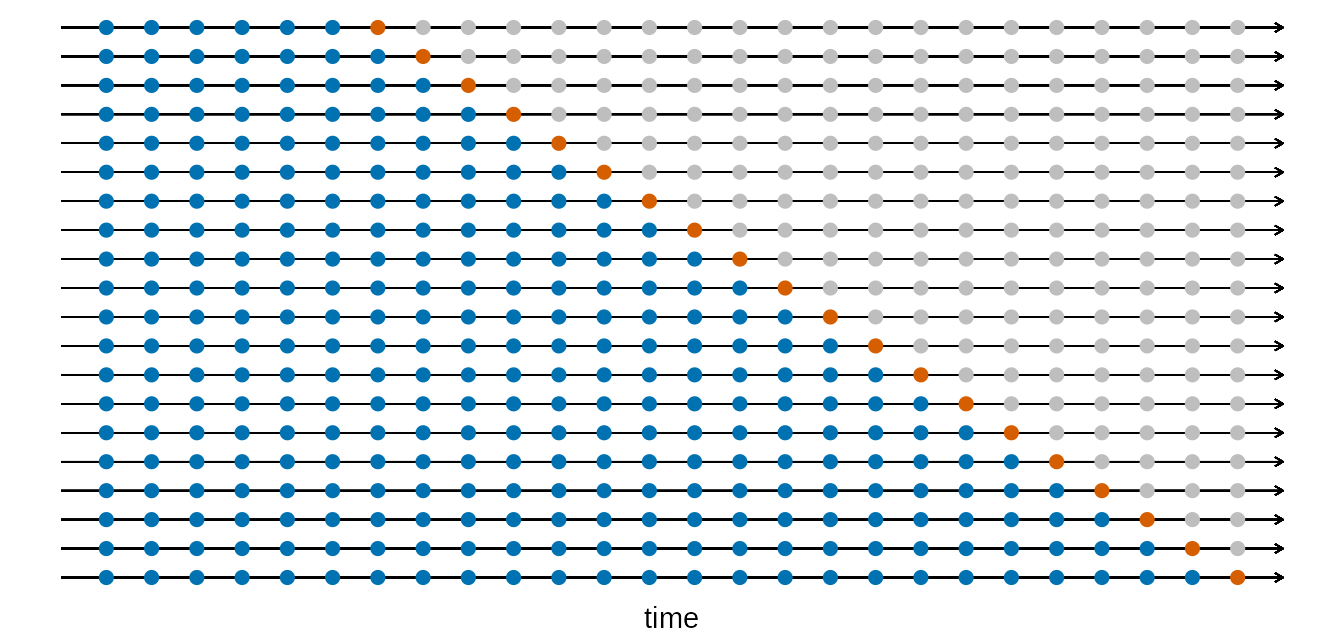
\includegraphics[width=\textwidth]{images/crossvalidationtimeseries.png}
    \caption{Cross validation for one step ahead timeseries data \cite{hyndman2018forecasting}}
    \label{fig:crossvalidationtimeseries}
\end{figure}
We then average all the observed losses in order to get an estimate for $Err$.
Notice, in the literature this procedure is sometimes also referred to evaluation on a rolling forecasting origin. This comes from the fact that at each iteration we push forward the origin of our forecast.
The same concept applies for multi step ahead forecasting, see picture \ref{fig:crossvalidationtimeseries2}.
That is in predicting $\hat{L}_{N+m}$ we use as inputs $L_1, L_2, \dots, \hat{L}_{N},\hat{L}_{N+1},\dots, \hat{L}_{N+m-1}$; where $\hat{L}_{N},\hat{L}_{N+1},\dots, \hat{L}_{N+m-1}$ are one step ahead forecasts.
\begin{figure}
    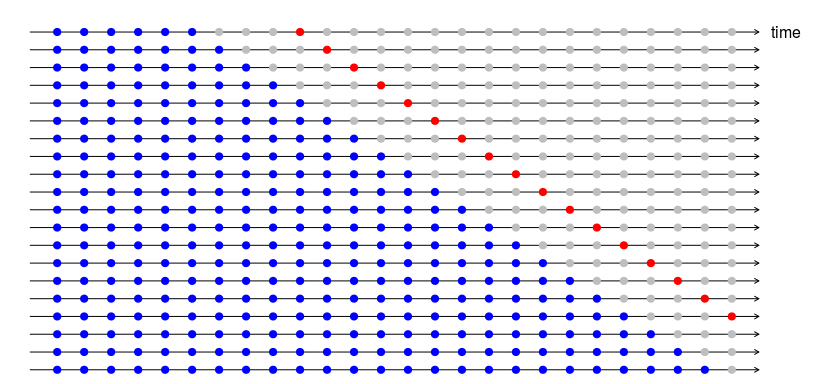
\includegraphics[width=\textwidth]{images/crossvalidationtimeseries2.png}
    \caption{Cross validation for m step ahead timeseries data \cite{hyndman2018forecasting}}
    \label{fig:crossvalidationtimeseries2}
\end{figure}

\section{Kernel methods best practices}
Following, are reported a couple of considerations important to keep in mind when working with kernel methods.

\subsection{Data normalization}\label{appendix:normalization}
With data normalization we transform the range of the feautures to a standard scale.
Such preprocessing step is essential when employing distance based algorithms like svm or k-nearest neighbors. The rationale behind it is that by normalizing data we give an uniform weight to each feature in the learning process; in this way we do not favour larger scale features.
Examples of the most popular features scaling are:
\begin{itemize}
    \item Standard scaler= it computes the standard score z of a sample x
    \\
    z=$\frac{x-\mu}{\sigma}$.
    \item MinMax scaler= it maps every data sample to the range 0, 1.
    \\
    $\frac{x-\min(X)}{\max(X)-\min(X)}$
    \item Robust scaler= it scales features using statistics that are robust to outliers.
    Essentially, it subtracts the median and then scales the data according to the interquantile range.
\end{itemize}
Many other data scaling algorithms exists, we refer the reader to a thorough comparison \cite{scikitscalers}.
\\
We conclude this subsection with a custom example that motivates the need of feature scaling \cite{scikitscale_example}. The idea is to compare the results of modelling the data with k nearest neighbors on the unscaled data against the scaled data. The considered data is the wine recognition dataset \href{https://archive.ics.uci.edu/dataset/109/wine}{https://archive.ics.uci.edu/dataset/109/wine}. The goal for this dataset is recognising from whose cultivator the wine comes based on two features with a completely different scale. The first feature has values in the [0,1000] range while the second feature has values contained in [1,10].
The unscaled and scaled version are compared in figure \ref{fig:feature_scaler_example}
\begin{figure}[!h]
    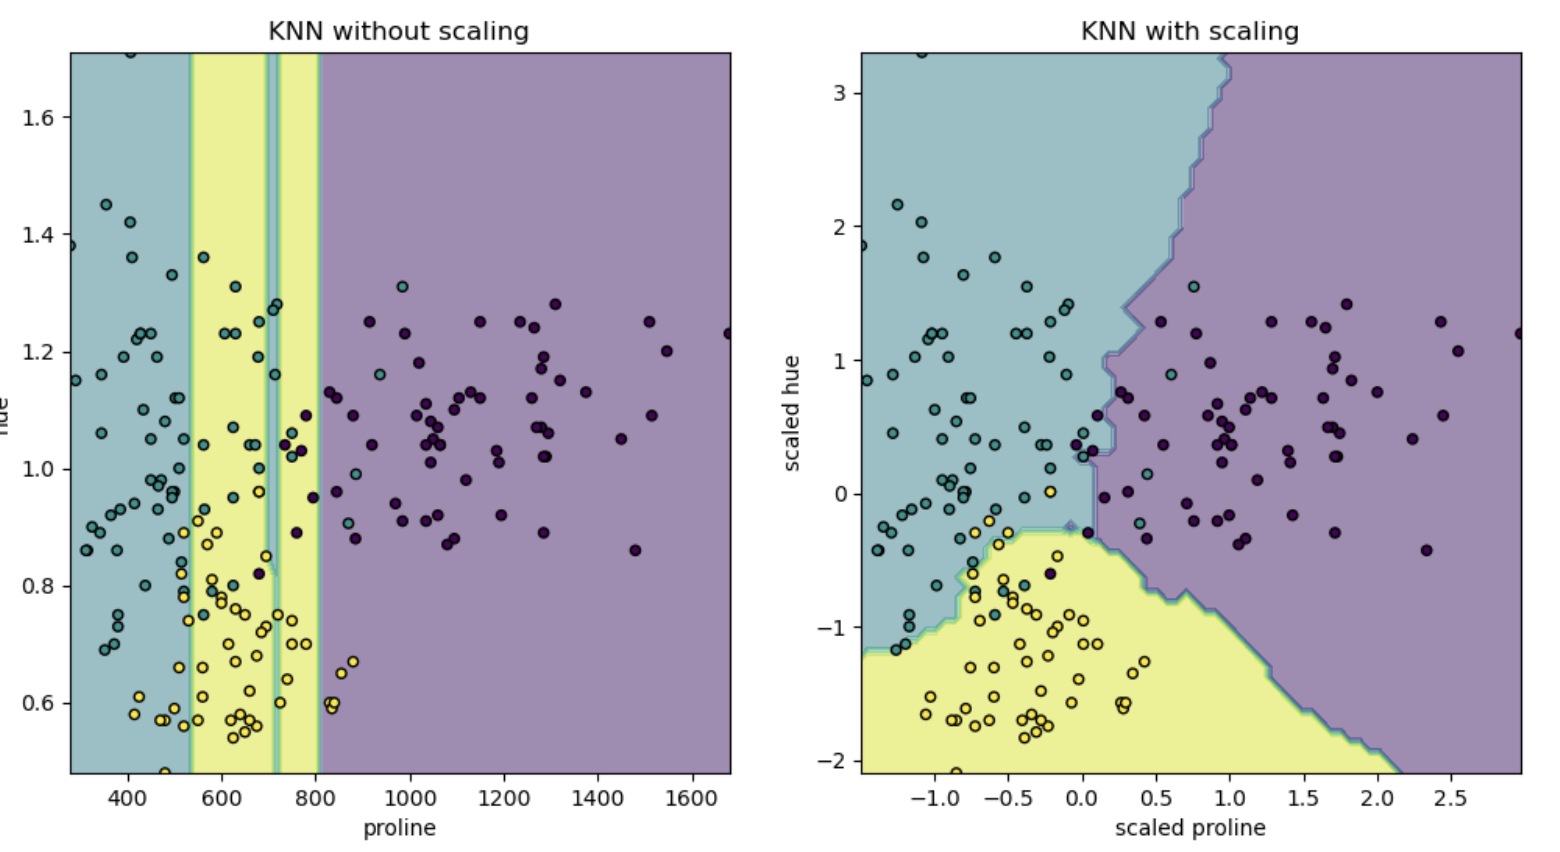
\includegraphics[width=\textwidth]{images/feature_scaler_example.png}
    \caption{importance of feature scaling}
    \label{fig:feature_scaler_example}
\end{figure}
What we can conclude from the image is that, the model trained on scaled data is greatly better than the other.
On the left, we can see that distances between categories are impacted solely by the larger scale feature. Conversely, on the right, we have that the two features contributing equally in determining the neighbors.

\subsection{Data compression}
When the number of points n is large, kernel methods suffer from high computational costs. 
Using kernel methods, we have that the storage cost is of the order of $O(n^2)$ while the computational cost for finding the solution is of the order $O(n^3)$.
A significant speed up can be obtained thanks to low rank approximation.


\subsubsection{Nystrom decomposition}
The Nyström approximation involves storing a submatrix of the whole kernel matrix. Thus, storage and computational cost are reduced to $O(nm)$ and $O(nm^2)$ respectively.
Nyström works by selecting $m<n$ points, callled representative points; it approximates K as
\begin{equation}
    \tilde {K}=K_{n,m} K_{m,m}^{-1}K_{n,m}^\intercal
\end{equation}


\subsubsection{Pivoted Cholesky decomposition}
Pivoted Cholesky approximate the Cholesky decomposition of a matrix. Since kernel matrices are positive definite, they can decomposed in terms of the Cholesky decomposition. Hence, we have that pivoted Cholesky can be used to approximate the full kernel matrix.


\newpage
\section{Src code}\label{src_code}
The whole code for the project is hosted on
\url{https://github.com/luca-pernigo/ThesisKernelMethods}\label{github_repo}.
\\
\begin{itemize}
    \item query: folder containing Scopus data and scripts to generate bibliometric survey plots in section \ref{literature_review}
    \item kqr.py: file implementing our custom kernel quantile regression
\end{itemize}


\backmatter

\bibliographystyle{plain}
\bibliography{refs}

% %Include all references
\nocite{*}


\end{document}
